% -*- Mode:TeX -*-

%% IMPORTANT: The official thesis specifications are available at:
%%            http://libraries.mit.edu/archives/thesis-specs/
%%
%%            Please verify your thesis' formatting and copyright
%%            assignment before submission.  If you notice any
%%            discrepancies between these templates and the 
%%            MIT Libraries' specs, please let us know
%%            by e-mailing thesis@mit.edu

%% The documentclass options along with the pagestyle can be used to generate
%% a technical report, a draft copy, or a regular thesis.  You may need to
%% re-specify the pagestyle after you \include  cover.tex.  For more
%% information, see the first few lines of mitthesis.cls. 

%\documentclass[12pt,vi,twoside]{mitthesis}
%%
%%  If you want your thesis copyright to you instead of MIT, use the
%%  ``vi'' option, as above.
%%
%\documentclass[12pt,twoside,leftblank]{mitthesis}
%%
%% If you want blank pages before new chapters to be labelled ``This
%% Page Intentionally Left Blank'', use the ``leftblank'' option, as
%% above. 

\documentclass[12pt,twoside]{mitthesis}
\usepackage{lgrind}
\usepackage{amssymb}
\usepackage{amsmath}
\usepackage{amsthm}
\usepackage{graphicx}
\usepackage{xcolor}
%% These have been added at the request of the MIT Libraries, because
%% some PDF conversions mess up the ligatures.  -LB, 1/22/2014
\usepackage{cmap}
\usepackage[T1]{fontenc}

\usepackage{setspace}
\doublespacing

\allowdisplaybreaks

\newtheorem{theorem}{THEOREM}[chapter]
\newtheorem{corollary}{COROLLARY}[theorem]
\newtheorem{lemma}{LEMMA}[theorem]

\theoremstyle{proposition}
\newtheorem{proposition}{PROPOSITION}[chapter]

\theoremstyle{remark}
\newtheorem{remark}{REMAEK}[chapter]

\theoremstyle{definition}
\newtheorem{definition}{DEFINITION}[chapter]

\newcommand\tobeclarified[1]{\textcolor{red}{#1}}
\newcommand\numberthis{\addtocounter{equation}{1}\tag{\theequation}}

\pagestyle{plain}

%% This bit allows you to either specify only the files which you wish to
%% process, or `all' to process all files which you \include.
%% Krishna Sethuraman (1990).

\typein [\files]{Enter file names to process, (chap1,chap2 ...), or `all' to
process all files:}
\def\all{all}
\ifx\files\all \typeout{Including all files.} \else \typeout{Including only \files.} \includeonly{\files} \fi

\begin{document}

% -*-latex-*-
% 
% For questions, comments, concerns or complaints:
% thesis@mit.edu
% 
%
% $Log: cover.tex,v $
% Revision 1.8  2008/05/13 15:02:15  jdreed
% Degree month is June, not May.  Added note about prevdegrees.
% Arthur Smith's title updated
%
% Revision 1.7  2001/02/08 18:53:16  boojum
% changed some \newpages to \cleardoublepages
%
% Revision 1.6  1999/10/21 14:49:31  boojum
% changed comment referring to documentstyle
%
% Revision 1.5  1999/10/21 14:39:04  boojum
% *** empty log message ***
%
% Revision 1.4  1997/04/18  17:54:10  othomas
% added page numbers on abstract and cover, and made 1 abstract
% page the default rather than 2.  (anne hunter tells me this
% is the new institute standard.)
%
% Revision 1.4  1997/04/18  17:54:10  othomas
% added page numbers on abstract and cover, and made 1 abstract
% page the default rather than 2.  (anne hunter tells me this
% is the new institute standard.)
%
% Revision 1.3  93/05/17  17:06:29  starflt
% Added acknowledgements section (suggested by tompalka)
% 
% Revision 1.2  92/04/22  13:13:13  epeisach
% Fixes for 1991 course 6 requirements
% Phrase "and to grant others the right to do so" has been added to 
% permission clause
% Second copy of abstract is not counted as separate pages so numbering works
% out
% 
% Revision 1.1  92/04/22  13:08:20  epeisach

% NOTE:
% These templates make an effort to conform to the MIT Thesis specifications,
% however the specifications can change.  We recommend that you verify the
% layout of your title page with your thesis advisor and/or the MIT 
% Libraries before printing your final copy.
\title{q-TASEP From the Duality Approach}

\author{Wang Kunzhen}
% If you wish to list your previous degrees on the cover page, use the 
% previous degrees command:
%       \prevdegrees{A.A., Harvard University (1985)}
% You can use the \\ command to list multiple previous degrees
%       \prevdegrees{B.S., University of California (1978) \\
%                    S.M., Massachusetts Institute of Technology (1981)}
\department{Department of Mathematics, Faculty of Science}


\homefaculty{Department of Computer Science, School of Computing}

% If the thesis is for two degrees simultaneously, list them both
% separated by \and like this:
% \degree{Doctor of Philosophy \and Master of Science}
\degree{Bachelor of Science (Hons) in Applied Mathematics}

% As of the 2007-08 academic year, valid degree months are September, 
% February, or June.  The default is June.
\degreemonth{March}
\degreeyear{2016}
\thesisdate{March, 2016}

%% By default, the thesis will be copyrighted to MIT.  If you need to copyright
%% the thesis to yourself, just specify the `vi' documentclass option.  If for
%% some reason you want to exactly specify the copyright notice text, you can
%% use the \copyrightnoticetext command.  
%\copyrightnoticetext{\copyright IBM, 1990.  Do not open till Xmas.}

% If there is more than one supervisor, use the \supervisor command
% once for each.
\supervisor{Wang Dong}{Assistant Professor}

% This is the department committee chairman, not the thesis committee
% chairman.  You should replace this with your Department's Committee
% Chairman.
%\chairman{Arthur C. Smith}{Chairman, Department Committee on Graduate Theses}

% Make the titlepage based on the above information.  If you need
% something special and can't use the standard form, you can specify
% the exact text of the titlepage yourself.  Put it in a titlepage
% environment and leave blank lines where you want vertical space.
% The spaces will be adjusted to fill the entire page.  The dotted
% lines for the signatures are made with the \signature command.
\maketitle

% The abstractpage environment sets up everything on the page except
% the text itself.  The title and other header material are put at the
% top of the page, and the supervisors are listed at the bottom.  A
% new page is begun both before and after.  Of course, an abstract may
% be more than one page itself.  If you need more control over the
% format of the page, you can use the abstract environment, which puts
% the word "Abstract" at the beginning and single spaces its text.

%% You can either \input (*not* \include) your abstract file, or you can put
%% the text of the abstract directly between the \begin{abstractpage} and
%% \end{abstractpage} commands.

% First copy: start a new page, and save the page number.
\cleardoublepage
% Uncomment the next line if you do NOT want a page number on your
% abstract and acknowledgments pages.
% \pagestyle{empty}
\setcounter{savepage}{\thepage}
\begin{abstractpage}
% $Log: abstract.tex,v $
% Revision 1.1  93/05/14  14:56:25  starflt
% Initial revision
% 
% Revision 1.1  90/05/04  10:41:01  lwvanels
% Initial revision
% 
%
%% The text of your abstract and nothing else (other than comments) goes here.
%% It will be single-spaced and the rest of the text that is supposed to go on
%% the abstract page will be generated by the abstractpage environment.  This
%% file should be \input (not \include 'd) from cover.tex.
In this thesis, I studied the model q-TASEP from the duality approach with main reference to the two papers \cite{duality2014} and \cite{asymptotics2013}. An ansatz explicit formula for the expectation of q-Laplace transform of the probability function describing the position of a particular particle at any time in the future in form of the nested contour integral will be provided. After this, I worked to transform a generating function of the nested contour integrals to the form of a Fredholm determinant using both the Mellin-Barnes type approach and the Cauchy-type approach. The thesis is then concluded with an asymptotic analysis on the behaviour of the rescaled fluctuation of a particular particle around its macroscopic position.
\end{abstractpage}

% Additional copy: start a new page, and reset the page number.  This way,
% the second copy of the abstract is not counted as separate pages.
% Uncomment the next 6 lines if you need two copies of the abstract
% page.
% \setcounter{page}{\thesavepage}
% \begin{abstractpage}
% % $Log: abstract.tex,v $
% Revision 1.1  93/05/14  14:56:25  starflt
% Initial revision
% 
% Revision 1.1  90/05/04  10:41:01  lwvanels
% Initial revision
% 
%
%% The text of your abstract and nothing else (other than comments) goes here.
%% It will be single-spaced and the rest of the text that is supposed to go on
%% the abstract page will be generated by the abstractpage environment.  This
%% file should be \input (not \include 'd) from cover.tex.
In this thesis, I studied the model q-TASEP from the duality approach with main reference to the two papers \cite{duality2014} and \cite{asymptotics2013}. An ansatz explicit formula for the expectation of q-Laplace transform of the probability function describing the position of a particular particle at any time in the future in form of the nested contour integral will be provided. After this, I worked to transform a generating function of the nested contour integrals to the form of a Fredholm determinant using both the Mellin-Barnes type approach and the Cauchy-type approach. The thesis is then concluded with an asymptotic analysis on the behaviour of the rescaled fluctuation of a particular particle around its macroscopic position.
% \end{abstractpage}

\cleardoublepage

\section*{Acknowledgments}

I would like to take the opportunity to express my special thanks to my supervisor, Professor Wang Dong, for his extraordinary support and assisstance extended to me for whole the year.

%%%%%%%%%%%%%%%%%%%%%%%%%%%%%%%%%%%%%%%%%%%%%%%%%%%%%%%%%%%%%%%%%%%%%%
% -*-latex-*-

% Some departments (e.g. 5) require an additional signature page.  See
% signature.tex for more information and uncomment the following line if
% applicable.
% % -*- Mode:TeX -*-
%
% Some departments (e.g. Chemistry) require an additional cover page
% with signatures of the thesis committee.  Please check with your
% thesis advisor or other appropriate person to determine if such a 
% page is required for your thesis.  
%
% If you choose not to use the "titlepage" environment, a \newpage
% commands, and several \vspace{\fill} commands may be necessary to
% achieve the required spacing.  The \signature command is defined in
% the "mitthesis" class
%
% The following sample appears courtesy of Ben Kaduk <kaduk@mit.edu> and
% was used in his June 2012 doctoral thesis in Chemistry. 

\begin{titlepage}
\begin{large}
This doctoral thesis has been examined by a Committee of the Department
of Chemistry as follows:

\signature{Professor Jianshu Cao}{Chairman, Thesis Committee \\
   Professor of Chemistry}

\signature{Professor Troy Van Voorhis}{Thesis Supervisor \\
   Associate Professor of Chemistry}

\signature{Professor Robert W. Field}{Member, Thesis Committee \\
   Haslam and Dewey Professor of Chemistry}
\end{large}
\end{titlepage}


\pagestyle{plain}
  % -*- Mode:TeX -*-
%% This file simply contains the commands that actually generate the table of
%% contents and lists of figures and tables.  You can omit any or all of
%% these files by simply taking out the appropriate command.  For more
%% information on these files, see appendix C.3.3 of the LaTeX manual. 
\tableofcontents
\newpage
\listoffigures
\newpage
\listoftables


%% This is an example first chapter.  You should put chapter/appendix that you
%% write into a separate file, and add a line \include{yourfilename} to
%% main.tex, where `yourfilename.tex' is the name of the chapter/appendix file.
%% You can process specific files by typing their names in at the 
%% \files=
%% prompt when you run the file main.tex through LaTeX.
\chapter{Introduction}
In this thesis I studied a 1-dimensional interacting particle system model called q-TASEP. It's one of the most recently yet classical particle model in this field that has important application in the physical world. For example, the model can be used to study mass transport, traffic flow and queuing behaviour etc. The article is concerned with the asymptotic behavior of the particles and is going to provide an explicit formulat describing the behavior. The approach starts from the duality between the q-TASEP model and another model called q-TAZRP. 

We are going to define the two model, q-TASEP and q-TAZRP in this chapter, and show some calculations of the q-TASEP from elementary approach. After this prove their duality in \textit{Chapter 2}. Then we provide an ansatz explicit formula for the expectation of q-Laplace transform of the probability function describing the position of a particular particle at any time in the future in form of the nested contour integral. In the chapter that follows we work to transform a generating function of the nested contour integral we have obtained into the form of a Fredholm determinant, using two different approaches. Lastly in \textit{Chapter 4} we perform asymptotic analysis to the Fredholm determinant and conclude that the rescaled fluctuation of the particle around the macroscopic follows a GUE Tracy-Widom distribution.

\section{Introduction to q-TASEP}
\label{sec:intro-qtasep}

q-TASEP, short for q-deformed totally asymmetric simple exclusion process, refers to a continuous time, discrete space Markov Process $\vec{x}(t)$ describing the dynamics of the following interacting particle system:

\begin{itemize}
\item Particles denoted by $\{x_1, x_2, x_3, ...\}$ occupy sites of $\mathbb{Z}$ exclusively with positions at time $t$ denoted as $x_i(t)$. The particles are ordered in such a way that $x_i(t) < x_j(t)$ for $i > j$.
\item Particles jump to the right by one spot ($x_i(t)$ increases by $1$) with jump rate given by $a_i (1-q^{x_{i-1}(t)-x_i(t)+1})$ for $i \ge 2$, where $q \in [0,1)$, $a_i > 0$. The jump rate for the particle $x_1$ is defined to be $a_1$.
\item All jumps occur indenpendently of each other according to exponential clocks with parameter $1$.
\end{itemize}

\begin{figure}
	\centering
	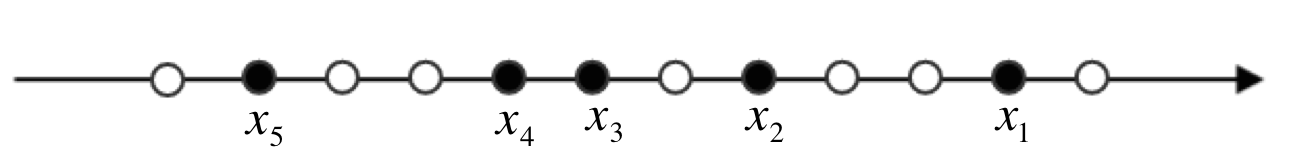
\includegraphics[width=0.5\textwidth]{q-TASEP}
	\caption[An illustration of q-TASEP]
	{An illustration of q-TASEP. The jump rate of the particle $x_2$ is given by $a_2(1-q^2)$, while that of the particle $x_4$ is $0$.}
	\label{fig:q-TASEP}
\end{figure}

It's worth noting that the ordering of the particles remains unchanged throughout the process. Note also that in the definition of q-TASEP, numbering of the particles starts with $1$. However, to facilitate our discussion, we could have added a virtual partical $x_0$ with $x_0 = \infty$ so that the jump rate of $x_1$ is also equal to $a_1 (1-q^{x_0(t) - x_1(t) + 1}) = a_1$. 

It can be easily seen that dynamics of the right most $N$ particles, i.e., particle $x_1$, $x_2$, $\dots$, $x_N$, is independent from those to the left of them, i.e., $x_{N+1}$, $x_{N+2}$, $\dots$ Therefore, from now onwards, we will be focusing on the study of q-TASEP with $N$ particles, with configuration $x_1(t) > x_2(t) > \dots > x_N(t)$. We could then define our state space as $$X^N = \{\vec{x}=(x_0,x_1,\dots, x_N) \in \{\infty \} \times \mathbb{Z}^N : \infty = x_0 > x_1 > \dots > x_N \}.$$

For q-TASEP with $N$ particles, the infinitesimal generator of $\vec{x}(t)$ acting on suitable function $f: X^N \rightarrow \mathbb{R}$, denoted by $L^{q-TASEP} f$, is given by $$(L^{q-TASEP} f) (\vec{x}) = \sum_{i=1}^{N} a_i (1-q^{x_{i-1} - x_i - 1}) (f(\vec{x}_i^{+}) - f(\vec{x})),$$ where $\vec{x}_i^{+}$ denotes the configuration of the q-TASEP with particle $x_i$ jumps to the right by $1$ position, i.e., $\vec{x}_i^+ = (x_0, x_1, \dots, x_{i-1}, x_i+1, x_{i+1}, \dots, x_N)$. This follows from the fact that for $t$ small, there is only $1$ chance for one of the $N$ particles to jump according its own jump rate.

\section{Initial data for q-TASEP}
For a q-TASEP to be well defined, additional to the dynamics of q-TASEP described in Section \ref{sec:intro-qtasep}, we also need an initial configuration of the process, called initial data. In this paper, we focus on two types of initial data, namely, the step initial data and the half stationary initial data. 

Step initial data is defined as the configuration of $x_i(0) = -i$ for $1 \le i \le N$. For half stationary initial data, we define q-Geometric distribution. 

\begin{definition}
\label{def:qgeo}
For $\alpha \in [0,1)$, we say that a random variable $X$ follows the q-Geometric distribution with parameter $\alpha$ [written as $X \sim qGeo(\alpha)$] if $$\mathbb{P}(X = k) = (\alpha;q)_{\infty} \frac{\alpha^k}{(q;q)_k},$$ where $(a;q)_n = (1-a)(1-aq)(1-aq^2)\dots(1-aq^{n-1})$ and $(a;q)_{\infty} = (1-a)(1-aq)(1-aq^2)\dots$
\end{definition}

Let $X_i \sim qGeo(\alpha/a_i)$ for $1 \le i \le N$ be $N$ independent q-Geometric random variables. Then the half stationary initial condition is defined recursively by first setting $x_1(0) = -1 + X_1$ and letting $x_i(0) = -1 + x_{i-1}(0) + X_i$ for $i > 1$. Note that when $\alpha = 0$, the step initial data is recovered.

\section{q-TASEP for a few particles}
The main goal for the study of q-TASEP in this thesis is to identify an exact formula for the distribution of the particle positions, $\mathbb{P}(x_N(t) = m)$ for $m \in \mathbb{Z}$ with step and half stationary initial data. In this section, we provide some intuitions of how this problem can be approached via elementary methods for q-TASEP of $1$ and $2$ particles, thereby illustrating how the complexity grows for $N$ large. 

\subsection{q-TASEP with $1$ particle}
In this section we focus on the q-TASEP with only $1$ particle denoted by $x_1$ starting at position $x_1(0) = 0$. Let $T_i$, $i = 1,2,\dots$ be independent and identically distributed exponential random variables with parameter $1$ denoting the time between the $(i-1)th$ and the $ith$ jump. For $m \in \mathbb{Z}_{\ge 0}$, define $$a_m = \mathbb{P}(x_1(t) \le m) = \mathbb{P}(\sum_{i=1}^{m+1} T_i > t)$$ such that $\mathbb{P}(x_1(t) = m) = a_m - a_{m-1}$ for $m \ge 1$ and $\mathbb{P}(x_1(t) = 0) = a_0 = e^{-t}$. Since $T_i \sim exp(1)$, $\sum_{i=1}^{m} T_i \sim Erlang(m,1)$ and therfore, by the density function of Erlang distribution, $$1 - a_m = \int_0^t \frac{s^m}{m!} e^{-s} ds.$$ 

\begin{proposition}
For q-TASEP with one particle $x_1$ with jump rate parameter $a_1 = 1$ and initial profile at $x_1(0) = -1$, we have that $\mathbb{E}[x_1(t)+1] = t$ and $\mathbb{E}[q^{x_1(t)+1}] = e^{(q-1)t}$.
\end{proposition}

\begin{proof}
From the notations above, we have that $\mathbb{P}(x_1(t) = m) = c_m - c_{m-1}$, where $c_m$ is defined by $c_m = 1 - \int_0^t \frac{s^m}{m!} e^{-s} ds$. Therefore, we have
\begin{align*}
\mathbb{E}[x_1(t)] &=  \lim_{n \to \infty} ((1-c_0) + (1-c_1) + ... + (1-c_{n-1}) - n ( 1-c_n))\\
  						&= \lim_{n \to \infty} (\int_{0}^{t} e^{-s}  (\sum_{i=0}^{n-1} \frac{s^i}{i!}) ds) +\lim_{n \to \infty} (n \times \int_{0}^{t} \frac{s^n}{n!} e^{-s} ds)\\
						&=  \int_{0}^{t} e^{-s} \lim_{n \to \infty} (\sum_{i=0}^{n-1} \frac{s^i}{i!}) ds + 0\\
						&=  \int_{0}^{t} e^{-s} e^s dt\\
						&= t
\end{align*}
Moreover, $\mathbb{E}[q^{x_0(t)}]$ can be computed as below: 
\begin{align*}
\mathbb{E}[q^{x_0(t)}] &= \lim_{n \to \infty} (q^0  c_0 + \sum_{i=1}^{n} q^i (c_i - c_{i-1}) )\\
											 &= \lim_{n \to \infty} (-(1-q) (\sum_{i=0}^{n-1} q^i (1-a_i)) - q^n (1-c_n) + 1)\\
											 &= - (1-q) \lim_{n \to \infty} ( \int_{0}^{t} e^{-s} \sum_{i=0}^{n-1} q^i \frac{s^i}{i!} ds) - \lim_{n \to \infty} \int_0^t q^n \frac{s^n}{n!} ds + 1\\
											 &=  - (1-q) \int_0^t e^{-s }  \lim_{n \to \infty} \sum_{i=0}^{n-1} q^i \frac{s^i}{i!} ds- \lim_{n \to \infty} \int_0^t q^n \frac{s^n}{n!} ds + 1\\
				     					 &=  - (1-q) \int_0^t e^{-s } e^{qs}  ds -\lim_{n \to \infty}  \int_0^t q^n \frac{s^n}{n!} ds + 1\\
				     					 &= e^{(q-1)t}.
\end{align*}
\end{proof}

\subsection{q-TASEP with $2$ particles}
Elementary methods similar to the one adopted for the one-particle system were applied for the $2$ particles system, and it was realized that the computation grew so complicated that nearly no conclusions was reached. Therefore, a different approach, namely the Komogorov Equation, was used to carry out the computation. Although no final conclusion was reached either at the end, some interesting results were found. 

Let us consider the two particles labeled as $x_1$ and $x_2$ starting at the initial positions that $x_1(0) = 0$ and $x_2(0) = a << 0$. Let $\mathbb{P}_{k,j}(t) = \mathbb{P}(x_1(t) = k, x_2(t) = j)$. We begin by giving the Komogorov Equation for the problem:
$$\frac{d}{dt} \mathbb{P}_{k,j}(t) = - \mathbb{P}_{k,j}(t) - (1-q^{k-j-1})\mathbb{P}_{k,j}(t) + (1-q^{k-j})\mathbb{P}_{k,j-1}(t) + \mathbb{P}_{k-1,j}(t)$$
with base cases  $\mathbb{P}_{k,j}(t) = 0$ if $j < a$ or $k < 0$ or $j \ge k$.\\
We will be applying induction on $k$ and $j$ separately, starting by iterating through $k = 0, 1, 2, \dots$. The result is stated as a proposition.
\begin{proposition}
With the notations and setting introduced above, for $m \ge 1$
 $$ \mathbb{P}_{m,a}(t) =\frac{1}{2 \pi i} \oint_{all poles} \frac{e^{(-2+z)t}}{(z-q^{-a-1})(z-q^{-a})...(z-q^{-a+m-1})} dz.$$
\end{proposition}
\begin{proof}
We will not be showing a complete proof here. Rather, we give some calculations for some base cases to check that the proposition is correct and provide some intuitions. \\
\textbf{Case 1}: For $k=0,j=a<0$, we have $$\frac{d}{dt} \mathbb{P}_{0,a}(t) + (2-q^{-a-1}) \mathbb{P}_{0,a}(t) = 0$$
 Solving this equation gives $$\mathbb{P}_{0,a}(t) = c e^{-(2-q^{-a-1})t}$$
 Notice that $\mathbb{P}_{0,a}(0) = 1$, then $c=1$. Therefore $$\mathbb{P}_{0,a}(t) = e^{-(2-q^{-a-1})t} = \frac{1}{2 \pi i} \oint_{all poles} \frac{e^{(-2+z)t}}{z-q^{-a-1}} dz$$
 \textbf{Case 2}: For $k=1, j=a<0$, we have $$\frac{d}{dt} \mathbb{P}_{1,a}(t) + (2-q^{-a}) \mathbb{P}_{1,a}(t) = e^{-(2-q^{-a-1})t}$$
 Therefore, $$\frac{d}{dt} [e^{(2-q^{-a})t} \mathbb{P}_{1,a}(t)] = e^{(q^{-a-1} - q^{-a})t}$$
 Solving this equation we have $$ \mathbb{P}_{1,a}(t) = \frac{e^{-(2-q^{-a-1})t}}{q^{-a-1} - q^{-a}} + c e^{-(2-q^{-a})t}$$
 Note that $\mathbb{P}_{1,a}(0) = 0$, we have $c = -\frac{1}{q^{-a-1} - q^{-a}}$ and therefore $$\mathbb{P}_{1,a}(t) = \frac{1}{q^{-a-1} - q^{-a}} (e^{-(2-q^{-a-1})t} - e^{-(2-q^{-a})t})$$
 In \textbf{contour integral} form, it can also be written as $$\mathbb{P}_{1,a}(t) =\frac{1}{2 \pi i} \oint_{all poles} \frac{e^{(-2+z)t}}{(z-q^{-a-1})(z-q^{-a})} dz$$
 \textbf{Case 3}: For $k=2, j=a<0$, we have $$\frac{d}{dt} \mathbb{P}_{2,a}(t) + (2-q^{1-a}) \mathbb{P}_{2,a}(t) = \mathbb{P}_{1,a}(t)$$
 Solving this equation gives 

 \begin{align*}
  \mathbb{P}_{2,a}(t) &= \frac{e^{(-2+q^{-a-1})t}}{ (q^{-a-1} - q^{-a})(q^{-a-1} - q^{1-a}) } - \frac{ e^{(-2+q^{-a})t} }{ (q^{-a-1} - q^{-a}) (q^{-a} - q^{1-a}) }\\
  & \quad + \frac{e^{(-2+q^{-a+1})t}}{ (q^{-a-1} - q^{-a+1})(q^{-a} - q^{-a+1}) } \\
  &=\frac{1}{2 \pi i} \oint_{all poles} \frac{e^{(-2+z)t}}{(z-q^{-a-1})(z-q^{-a})(z-q^{-a+1})} dz
 \end{align*}
\end{proof}
Next, we investigate the cases $k = 0, j = a, (a+1), \dots, -1$. The result is stated as the following proposition.
\begin{proposition}
With the notations and setting introduced above, for $k = 0, j = a+n$, $0 \le n < a$, we have \\
\begin{align*}
\mathbb{P}_{0,a+n} (t) &= \frac{(1-q^{-a-1})(1-q^{-a-2})...(1-q^{-a-n})}{2 \pi i} \\
& \quad \times \oint_{all poles} \frac{e^{(-2+z)t}}{(z-q^{-a-1})(z-q^{-a-2})...(z-q^{-a-n-1})} dz.
\end{align*}
\end{proposition}

\begin{proof}
Again, we will only be providing some intuitions regarding the equality. \\
For $k=0, j=a+1$, we have $$\frac{d}{dt} \mathbb{P}_{0,a+1}(t) + (2-q^{-a-2}) \mathbb{P}_{0,a+1}(t) = (1-q^{-a-1}) \mathbb{P}_{0,a}(t)$$
 Solving this equation gives 

 \begin{align*}
 \mathbb{P}_{0,a+1} (t) &= \frac{1-q^{-a-1}}{q^{-a-1} - q^{-a-2}} (e^{-(2-q^{-a-1})t} - e^{-(2-q^{-a-2})t})\\
 &= (1-q^{-a-1}) \frac{1}{2 \pi i} \oint_{all poles} \frac{e^{(-2+z)t}}{(z-q^{-a-1})(z-q^{-a-2})} dz
 \end{align*}
\end{proof}

More general application of induction on both $k$ and $j$ together was carried out and didn't reach any elegant results as the ones mentioned above. Therefore, the elementary calculation for the q-TASEP model was stopped and the focus was then turned to studying the duality approach. However, such calculations demonstrate how fast the complexity grows with the number of particles considered, and they were also important as they provided essential fundamental understanding of the model. 

\section{Introduction to q-TAZRP}
Next, we introduce another Markov process called q-TAZRP, short for q-deformed totally asymmetric zero range process. q-TAZRP on an interval $\{0,1,...,N\}$ is a continuous time, discrete space Markov process $\vec{y}(t)$ with state space $$Y^N = (\mathbb{Z}_{\ge 0})^{N+1}$$ subject to the condition of $\sum_{i=0}^{N} y_i(t) = \sum_{i=0}^{N} y_i(0)$ $\forall$ $t\in\mathbb{R}_{\ge 0}$. Dynamics of a q-TAZRP is defined as the following:
\begin{itemize}
\item For each $i \in \{1,2,\dots,N\}$, $y_i(t)$ decreases by $1$ and $y_{i-1}(t)$ increases by $1$ simultaneously according to a rate function given by $g_i(k) = a_i (1-q^{y_i(t)})$.
\item All changes occur independently for each site according to exponential clocks.
\item $y_0$ is always non-decreasing.
\end{itemize}

\begin{figure}
	\centering
	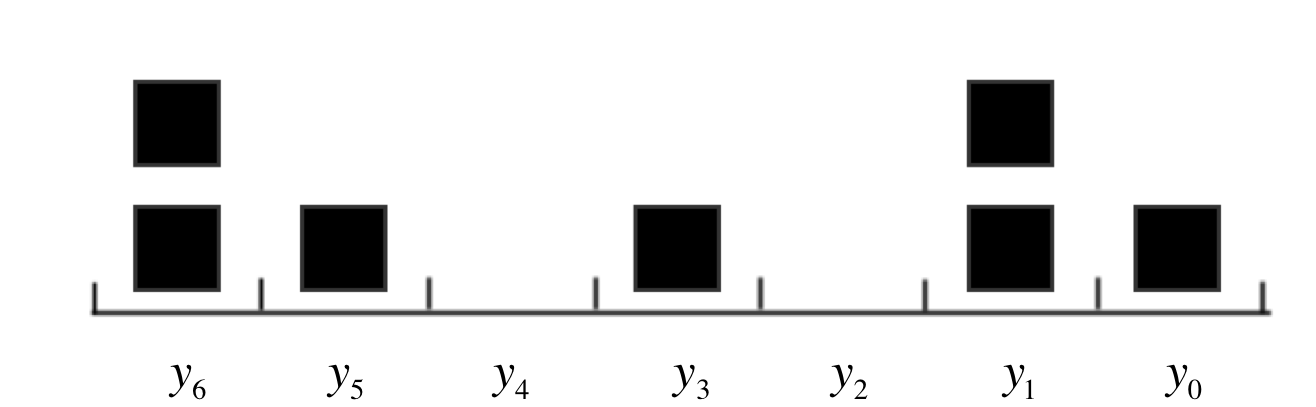
\includegraphics[width=0.75\textwidth]{q-TAZRP}
	\caption[An illustration of q-TAZRP]
	{An illustration of q-TAZRP. Rate function for site $y_1$ is given by $a_1 (1-q^2)$.}
	\label{fig:qTAZRP}
\end{figure}

A natural interpretation of the q-TAZRP is given in Figure \ref{fig:qTAZRP}, where a total of $\sum_{i=0}^{N} y_i(0)$ particles occupy the $N$ sites ordered in such a way that $y_i$ is to the left of $y_{i-1}$ for $i = 1,2,\dots,N$. The changes in the definition then refer to a jump of the top particle at site $y_i$ to the site $y_{i-1}$. Note then that no particle leaves site $0$.

It can be shown that the infinitesimal generator of $\vec{y}(t)$ acting on a suitable function $h:Y^N \rightarrow \mathbb{R}$, denoted as $L^{q-TAZRP} h$, is given by $$(L^{q-TAZRP} h)(\vec{y}) = \sum_{i=1}^{N} a_i (1-q^{y_i}) (h(\vec{y}^{i,i-1}) - h(\vec{y})),$$ where $\vec{y}^{i,i-1}$ represents the configuration of $(y_0, \dots, y_{i-2}, y_{i-1}+1, y_i - 1, y_{i+1}, \dots, y_N)$.

Lastly, we present another notation, $\vec{n} \in W^k_{>0}$, for the states of a q-TAZRP, where $W^k_{>0} = \{(n_1,n_2,\dots,n_k) \in (\mathbb{Z}_{>0})^k : n_1 \ge n_2 \ge \dots \ge n_k \ge 0 \}$. The vector $\vec{n}(\vec{y})$ for any state $\vec{y}$ of the q-TAZRP is given by $$y_i = \left| \{ n_j : n_j = i \} \right|.$$ The intuition is that while $y_i$ in $\vec{y}$ denotes the number of particles at site $i$, $n_j$ in $\vec{n}$ denotes the positioin of Particle $j$ ordered according to decreasing site locations. Take the configuration in Figure \ref{fig:qTAZRP} for example. Its representation in $\vec{y}$ is given by $\vec{y} = (1,2,0,1,0,1,2)$, while in $\vec{n}$ it is represented as $\vec{n} = (6,6,5,3,1,1,0)$. 

\chapter{Duality and Nested Contour Integral Ansatz Solution}
In this chapter, we recall the definition of duality between two Markov process defined in \cite{interacting-particle-system}. Then we prove the duality between q-TASEP and q-TAZRP. We then conclude by giving an ansatz solution for q-TASEP with step initial data as well as half stationary initial data. 

\section{Duality}
a
\section{Duality between q-TASEP and q-TAZRP}
a
\section{Evolution Equation Systems}
a
\section{Nested Contour Integral Solution}
a
\chapter{Fredholm Determinants}
In last chapter, we have derived a nested contour integral expression for $\mathbb{E}[\prod_{j=1}^k q^{x_{n_j}+n_j}]$ using some ODE systems. In this chapter we introduce Fredholm Determinants and try to transform the nested contour integrals into the form of a Fredholm determinants. However, from now onwards, we will only be focusing on the distribution of a single particle $x_n(t)$, since the joint distribution of an arbitrary collection of particles $x_{n_1}(t), \dots, x_{n_l}(t)$ will involve some further complexities that will bring challenges into getting a relatively simple expression. To do this, we apply Corollary \ref{nested-contour-corollary} with $\vec{n} = (n,n,\dots, n)$, which results in $\mathbb{E}[\prod_{j=1}^k q^{x_{n_j}+n_j}] = q^{kn} \mathbb{E} [q^{kx_n(t)}]$. 

\section{Fredholm Determinants}
We begin by quoting the definition of a Fredholm determinant from Definition 3.2.6 in \cite{macdonald2014}.

\begin{definition}
Fix a Hilbert space $L^2(X,\mu)$ where $X$ is a measurable space and $\mu$ is a measure on $X$. When $X = \Gamma$, a simple smooth contour in $\mathbb{C}$, we write $L^2(\Gamma)$ where $\mu$ is understood to be the path measure along $\Gamma$ divided by $2 \pi i$. When $X$ is the product of a discrete set $D$ and a contour $\Gamma$, $\mu$ is understood to be the product of the counting measure on $D$ and the path measure along $\Gamma$ divided by $2 \pi i$.
Let K be an integral operator acting on $f(\cdot) \in L^2(X,\mu)$ by $$(Kf)(x) = \int_X K(x,y) f(y) d\mu(y).$$ $K(x,y)$ is called the kernel of $K$. A formal Fredholm determinant expansion of $I+K$ is a formal series written as $$det(I+K) = 1 + \sum_{n=1}^{\infty} \frac{1}{n!} \int_X \dots \int_X det[K(x_i,x_j)]_{i,j=1}^{n} \prod_{i=1}^{n} d\mu(x_i)$$
If the above series is absolutely convergent, then we call this a numerical Fredholm determinant expansion.
\end{definition}

In order to transform a nested contour integrals of similar forms to the ones given in Theorem \ref{thm:nested-contour-integration}, the idea is to deform the nested contours so that they coincide. However, there are two types of deformation, namely the Mellin-Barnes type and the Cauchy type. The philosophy for the Mellin-Barnes type approach is to deform the contours in such a way that all of the poles corresponding to $z_A = qz_B$ for $A < B$ are encountered. This is, in some sense, shrinking the contours so that they coincide. The Cauchy type approach does the opporsite that it enlarges the contours so that they coincide. Poles at $z_k = 0$ are encountered in this process.

In the following sections, we introduce the two approaches in details and see how each of them can be applied to q-TASEP. But before that, we first identify the exact form of nested contours to be manipulated by Definition 3.1 in \cite{macdonald2014}.

\begin{definition}
\label{mu_k_def}
For a meromorphic function $f(z)$ and $k \ge 1$ set $\mathbb{A}$ to be a fixed set of poles of $f$ (not including 0) and assume that $q^m \mathbb{A}$ is disjoint from $\mathbb{A}$ for all $m \ge 1$. Define
$$\mu_k = \frac{(-1)^k q^{k(k-1)/2}}{(2 \pi i)^k} \int \dots \int \prod_{1 \le A < B \le k} \frac{z_A - z_B} {z_A - qz_B} \prod_{i=1}^k f(z_i) \frac{dz_i}{z_i},$$ where the integration contour for $z_A$ contains $\{qz_B\}_{B > A}$, the fixed set of poles $\mathbb{A}$ of $f(z)$ but not $0$ or any other poles. 
\end{definition}

Notice that when we take $f(z) = \left( \prod_{m=1}^{n} \frac{a_m}{a_m - z} \right) e^{(q-1)tz}$, $u(t;\vec{n})$ for step initial data in Theorem \ref{thm:nested-contour-integration} is recovered.

\section{Mellin-Barnes type determinants}

\subsection{Mellin-Barnes type transformation}
\label{m-b-type-transformation}
First, we introduce some notations used. For $\lambda = (\lambda_1 \ge \lambda_2 \ge \dots \ge 0)$, we write $\lambda \vdash k$ if $\sum_i \lambda_i = k$ and $\lambda = 1^{m_1} 2^{m_2} \dots$ if $i$ appears $m_i$ times in $\lambda$. Let $l(\lambda) = \sum_i m_i$ denote the number of non-zero elements of $\lambda$.\\

In Mellin-Barnes type determinants, the nested contours are deformed to coincide so that the only poles encountered are at $z_A = qz_B$ for $A < B$. With this philosophy, we transform the $\mu_k$ as defined in Definition \ref{mu_k_def} into the following form with the contours shrinked to coincide. The result is given in the following proposition.
\begin{proposition}
\label{mellin-barnes-transform}
Define
\begin{align*}
\gamma_k &= k_q! \sum_{\substack{{\lambda \vdash k}\\ {\lambda = 1^{m_1} 2^{m_2} \dots}}} \frac{1}{m_1! m_2! \dots} \frac{(1-q)^k}{(2 \pi i)^{l(\lambda)}} \\
			& \quad \times \int \dots \int det\left[ \frac{1}{w_iq^{\lambda_i} - w_j} \right]_{i,j=1}^{l(\lambda)} \times \prod_{j=1}^{l(\lambda)} f(w_j) f(qw_j) \dots f(q^{\lambda_j-1} w_j) dw_j \numberthis \label{new_mu_k}
\end{align*}
where the $w_j$ contours contain the same fixed set of singularities $\mathbb{A}$ of $f(z)$ but no other poles and $k_q! = \prod_{i=1}^{k} \frac{1-q^i}{1-q} = \frac{(q;q)_k}{(1-q)^k}$. Then for all $k \in \mathbb{Z} $,
$$\gamma_k = \mu_k$$
\end{proposition}

\begin{remark}
Note that in $\gamma_k$ the contours have been deformed to coincide with each other containing the same fixed set of singularities. 
\end{remark}

Before moving on to the proof, we discuss a transformation of the RHS of Equation \ref{mellin-barnes-transform}. \\
In $\gamma_k$, in order to evaluate the integral, for each $\lambda \vdash k$, we have to sum over all possible combination of $l(\lambda)$ poles chosen from the fixed set $\mathbb{A}$ of poles of $f(z)$. Because of the determinant, zero contribution would occur if identical poles were chosen for different variable $w_i \neq w_j$ since it would result in two identical columns in the determinant. Therefore, when considering a set of $l(\lambda)$ poles, we will make sure that the poles chosen are mutually distinct.

Moreover, for a particular $\lambda$ with some $\lambda_i = \lambda_j$ for $i \neq j$, interchanging $\lambda_i$ and $\lambda_j$ will not affect the evaluation. This allows us to cancel away the prefactor of $\frac{1}{m_1! m_2! \dots}$. Hence, we can replace the summation over $\lambda$ in Equation \ref{mellin-barnes-transform} by a summation over disjoint subsets of $\mathit{J}$ of size $m_1$, $m_2$, etc, where $m_1 + 2m_2 + \dots = k$. Denote these subsets by $S_1, S_2, \dots$ respectively and write $S = (S_1, S_2, \dots ) = (b_1, \dots, b_{m_1}, b_{m_1+1}, \dots, b_{m_1 + m_2}, \dots)$, where $b_i \in S_1$ for $1 \le i \le m_1$, $b_i \in S_2$ for $m_1 < i \le m_2$ and so on. Denote the set of all such collections of subsets $S's$ to be $\mathcal{S}$. Then by evaluating the corresponding residues Equation \ref{mellin-barnes-transform} can be transformed to
\begin{equation}
\gamma_k = \sum_{S \in \mathcal{S}} k_q! (1-q)^k \prod_{j=1}^{m_1+m_2+\dots} Res_{w=b_j} f(w) f(qb_j) \dots f(q^{\lambda(b_j)} b_j) det\left[ \frac{1}{b_iq^{\lambda(b_i)} - b_j} \right]_{i,j=1}^{m_1+m_2+\dots}
\end{equation}

To illustrate what has been discussed above, we take $k = 4$ for an example. In this case, all possible $\lambda 's$ are $(4,0), (3,1), (2,2), (2,1,1), (1,1,1,1)$. Take $\lambda = (2,1,1')$ (In $1'$ the superscript is to differentiate it from the previous $1$) and we get $m_1 = 2$, $m_2 = 1$, $m_i = 0$ for $i \ge 3$ and $l(\lambda) = 3$. Therefore, $|S_1| = m_1 = 2$ and $|S_2| = m_2 = 1$. One possible collection of such $S_i's$ is $S_1 = \{1,1'\}$ and $S_2 = \{2\}$ and hence $S = (\{1,1'\},  \{2\})$. Therefore, for this particular $k = 3$ and $\lambda$, all possible collections of such $S's$ are 
\begin{align}
\mathcal{S}_{\lambda} = \{ &(\{1,1'\},\{2\}), (\{1,2\},\{1'\}), \\ 
													 &(\{1',1\},\{2\}), (\{1', 2\},\{1\}),\\
													 &(\{2,1\},\{1'\}), (\{2,1'\},\{1\})\}
\end{align}
Notice that the sets $S's$ are ordered sets since they corresponds to poles of different $w_j's$. Also, notice that interchanging $1$ and $1'$ results in equal contributions. Therefore, the prefactor $\frac{1}{m_1! m_2! \dots} = \frac{1}{2}$ is needed to account for this effect.

\begin{proof}[Proof of Proposition \ref{mellin-barnes-transform}]
The proof is by induction on $k$. For $k=1$, by definition, 
$$\mu_1 = - \frac{1}{2 \pi i} \int f(z_1) \frac{dz_1}{z_1}.$$ Moreover, the only $\lambda$ is $\lambda = (1,0)$ and $\gamma_k$ reduces to $$\frac{1-q}{2 \pi i} \int \frac{1}{q w_1 - w_1 } f(w_1) dw_1 = - \frac{1}{2 \pi i} \int f(w_1) \frac{dw_1}{w_1}.$$ Comparing the two expression, we get that $\mu_1 = \gamma_1$.

For the induction step, let $k \in \mathbb{Z}_+$ and assume that $\mu_{k-1} = \gamma_{k-1}$. Let $\mathit{J}$ denote an index set of $\mathbb{A}$ $(\mathit{J} = \{1,\dots,|\mathbb{A}|\})$ and recall the definition of $\mu_k$ in Definition \ref{mu_k_def} that $$\mu_k = \frac{(-1)^k q^{k(k-1)/2}}{(2 \pi i)^k} \int \dots \int \prod_{1 \le A < B \le k} \frac{z_A - z_B} {z_A - qz_B} \prod_{i=1}^k f(z_i) \frac{dz_i}{z_i},$$ we evaluate the integral over $z_k$ using residue calculus to get
\begin{align*}
\mu_k &= (-q^{k-1}) \sum_{j \in \mathit{J}} \frac{Res_{z = a_j} f(z)}{a_j} (-1)^{k-1} \frac{q^{(k-1)(k-2)/2}}{(2 \pi i)^{k-1}} \\
& \quad \times \int \dots \int \prod_{1 \le A < B \le k-1} \frac{z_A - z_B}{z_A - qz_B} \prod_{i=1}^{k-1} \frac{z_i - a_j}{z_i - qa_j} \frac{f(z_i)}{z_i} dz_i. \numberthis \label{induction-mu}
\end{align*}
Notice that the integral on the right hand side of Equation \ref{induction-mu} is an $k-1$ fold nested contour integral, to which we can apply, for each $j$, our induction assumption with $\tilde{f}_j(z) = f(z) \frac{z-a_j}{z-qa_j}$ and the new sets of poles $\tilde{\mathbb{A}}_j = (\mathbb{A} \setminus \{a_j\}) \cup \{qa_j\}$. The resulting form is 
\begin{align*}
\mu_k &= (-q^{k-1}) \sum_{j \in \mathit{J}} \frac{Res_{z = a_j} f(z)}{a_j} \times (k-1)_q! \sum_{\substack{{\lambda \vdash k-1}\\ {\lambda = 1^{\tilde{m}_1} 2^{\tilde{m}_2} \dots}}} \frac{1}{\tilde{m}_1! \tilde{m}_2! \dots} \frac{(1-q)^{k-1}}{(2 \pi i)^{l(\lambda)}} \\
			& \quad \times \int \dots \int det\left[ \frac{1}{w_iq^{\lambda_i} - w_j} \right]_{i,j=1}^{l(\lambda)} \times \prod_{t=1}^{l(\lambda)} \tilde{f}_j(w_t) \tilde{f}_j(qw_t) \dots \tilde{f}_j(q^{\lambda_t-1} w_t) dw_t \numberthis \label{mu-form-2}
\end{align*}

From the transformation discussed just before the proof, we can see that (\ref{mu-form-2}) can be transformed to 
\begin{align*}
%\mu_k &= (-q^{k-1}) (k-1)_q! (1-q)^{k-1} \sum_{j \in \mathit{J}} \sum_{\tilde{S} \in \tilde{\mathcal{S}}_j} \frac{1}{a_j}  det\left[ \frac{1}{ \tilde{b}_i q^{\tilde{\lambda}(\tilde{b}_i)} - \tilde{b}_l } \right]_{\tilde{b}_i, \tilde{b}_l \in \tilde{S}}\\
%& \quad \times \prod_{\tilde{b} \in \tilde{S} \setminus \{qa_j\}} Res_{w = \tilde{b}} \tilde{f}_j(w) \tilde{f}_j(q\tilde{b}) \dots \tilde{f}_j(q^{\tilde{\lambda}(\tilde{b}) - 1} \tilde{b}) \\
%& \quad \times Res_{w = a_j} f(w) \times Res_{w = qa_j} \tilde{f}_j(w) \tilde{f}_j(q^2 a_j) \dots \tilde{f}_j(q^{\tilde{\lambda}(qa_j)} a_j) \numberthis \label{mu-form-3}
\mu_k &= (-q^{k-1}) (k-1)_q! (1-q)^{k-1} \sum_{j \in \mathit{J}} \sum_{\tilde{S} \in \tilde{\mathcal{S}}_j} \frac{1}{a_j}  det\left[ \frac{1}{ \tilde{b}_i q^{\tilde{\lambda}(\tilde{b}_i)} - \tilde{b}_l } \right]_{\tilde{b}_i, \tilde{b}_l \in \tilde{S}}\\
& \quad \times Res(\tilde{S}) \times Res_{w = a_j} f(w), \numberthis \label{mu-form-3}
\end{align*}
where for $\tilde{S}$ such that $qa_j \in \tilde{S}$,
\begin{align*}
Res(\tilde{S}) &= \prod_{\tilde{b} \in \tilde{S} \setminus \{qa_j\}} Res_{w = \tilde{b}} \tilde{f}_j(w) \tilde{f}_j(q\tilde{b}) \dots \tilde{f}_j(q^{\tilde{\lambda}(\tilde{b}) - 1} \tilde{b}) \\
& \quad \times Res_{w = qa_j} \tilde{f}_j(w) \tilde{f}_j(q^2 a_j) \dots \tilde{f}_j(q^{\tilde{\lambda}(qa_j)} a_j) \numberthis \label{mu-form-sub-3}
\end{align*}
and otherwise
$$Res(\tilde{S}) = \prod_{\tilde{b} \in \tilde{S}} Res_{w = \tilde{b}} \tilde{f}_j(w) \tilde{f}_j(q\tilde{b}) \dots \tilde{f}_j(q^{\tilde{\lambda}(\tilde{b}) - 1} \tilde{b}),
$$
where $\tilde{\mathcal{S}}_j$ denotes the set of all collections $\tilde{S}$ of subsets $\tilde{S}_{j,1}, \tilde{S}_{j,2}, \dots$ of $\tilde{\mathbb{A}}_j$, where $\tilde{S}_{j,k}$ is of size $\tilde{m}_k$ and $\tilde{m}_1 + 2\tilde{m}_2 + \dots = k-1$. Also, we reorder the elements in $\tilde{S}$ to be $\tilde{S} = (\tilde{b}_1, \tilde{b}_2, \dots, \tilde{b}_{\tilde{m}_1}, \dots)$ so that the first $\tilde{m}_1$ elements belong to $\tilde{S}_{j,1}$ etc.\\ \\
Note that for $\tilde{b} \neq a_j$ such that $\tilde{\lambda}(\tilde{b}) = \lambda$, 
\begin{align*}
&Res_{w=\tilde{b}} \tilde{f}_j(w) \tilde{f}_j(q\tilde{b}) \dots \tilde{f}_j(q^{\lambda-1} \tilde{b}) \\
& \quad= \frac{\tilde{b} - a_j}{\tilde{b} - qa_j} \frac{q\tilde{b} - a_j}{q\tilde{b} - qa_j} \dots \frac{q^{\lambda-1} \tilde{b} - a_j}{q^{\lambda-1} \tilde{b} - qa_j} Res_{w=\tilde{b}} f(w) f(q \tilde{b}) \dots f(q^{\lambda-1}\tilde{b}) \\
& \quad=  \frac{q^{\lambda - 1} \tilde{b} - a_j}{\tilde{b} - qa_j} q^{1 - \lambda} Res_{w = \tilde{b}} f(w) f(q\tilde{b}) \dots f(q^{\lambda-1} \tilde{b}) \numberthis \label{equality-mu-1}
\end{align*}
and 
\begin{align*}
& Res_{w = qa_j} \tilde{f}_j(w) \tilde{f}_j(q^2 a_j) \dots \tilde{f}_j(q^{\tilde{\lambda}(qa_j)} a_j)\\
& \quad = (q-1)a_j \frac{q^2a_j - a_j}{q^2 a_j - qa_j} \dots \frac{q^{\tilde{\lambda}(qa_j)}a_j - a_j}{q^{\tilde{\lambda}(qa_j)} a_j - qa_j} f(qa_j) \dots f(q^{\tilde{\lambda}(qa_j)} a_j) \\
& \quad = a_j (q^{\tilde{\lambda}(qa_j)} - 1) q^{2 - \tilde{\lambda}(qa_j)} f(qa_j) \dots f(q^{\tilde{\lambda}(qa_j)} a_j) \numberthis \label{equality-mu-2}
\end{align*}
Applying (\ref{equality-mu-1})  and (\ref{equality-mu-2}) to (\ref{mu-form-sub-3}), we get for $\tilde{b} \neq a_j$ such that $\tilde{\lambda}(\tilde{b}) = \lambda$,
\begin{align*}
Res(\tilde{S}) &= \prod_{\tilde{b} \in \tilde{S} \setminus \{qa_j\}} \frac{q^{\tilde{\lambda}(\tilde{b}) - 1} \tilde{b} - a_j}{\tilde{b} - qa_j} q^{1 - \tilde{\lambda}(\tilde{b})} Res_{w = \tilde{b}} f(w) f(q\tilde{b}) \dots f(q^{\tilde{\lambda}(\tilde{b})-1} \tilde{b}) \\
& \quad \times a_j (q^{\tilde{\lambda}(qa_j)} - 1) q^{2 - \tilde{\lambda}(qa_j)} f(qa_j) \dots f(q^{\tilde{\lambda}(qa_j)} a_j) \\
&= \prod_{l \neq j} \frac{q^{\tilde{\lambda}(b_l) - 1} b_l - a_j}{b_l - qa_j} q^{1 - \tilde{\lambda}(b_l)} Res_{w = b_l} f(w) f(qb_l) \dots f(q^{\tilde{\lambda}(b_l)-1} b_l) \\
& \quad \times a_j (q^{\tilde{\lambda}(qa_j)} - 1) q^{2 - \tilde{\lambda}(qa_j)} f(qa_j) \dots f(q^{\tilde{\lambda}(qa_j)} a_j)
\numberthis \label{mu-form-4}
\end{align*}
For convenience purpose, for each $\tilde{S} = (\tilde{S}_{j,1}, \tilde{S}_{j,2}, \dots) \in \tilde{\mathcal{S}}_j$, we map it to a new set $S_j = (S_{j,1}, S_{j,2}, \dots)$ in the following manner:\\
If $qa_j \in \tilde{S}_{j,l}$  for some $l$, then $$S_{j,l} = \tilde{S}_{j,l} \setminus \{qa_j\}, S_{j,l+1} = \tilde{S}_{j,l+1} \cup \{a_j\}, S_{j,m} = \tilde{S}_{j,m} \text{ for all } m \neq l, l+1,$$
Otherwise, $$S_{j,1} = \tilde{S}_{j,1} \cup \{a_j\}, S_m = \tilde{S}_m \text{ for all } m > 1.$$
With the new set $S_j$, we can then write $Res_{w=a_j} f(w) Res(\tilde{S})$ in the following form
\begin{align*}
Res_{w=a_j} f(w) Res(\tilde{S}) &= a_j (q^{\tilde{\lambda}(qa_j)} - 1) q^{2 - \tilde{\lambda}(qa_j)} \prod_{l \neq j}  \frac{q^{\tilde{\lambda}(b_l) - 1} b_l - a_j}{b_l - qa_j} q^{1 - \tilde{\lambda}(b_l)} \\
& \quad \times \prod_{b \in S_{j,1} \cup S_{j,2} \dots} Res_{w = b} f(w) f(qb) \dots f(q^{\tilde{\lambda}(b) - 1}b) \numberthis \label{always-true-set-transform}
\end{align*}
Notice that (\ref{always-true-set-transform}) always holds regardless of whether $qa_j$ is in $\tilde{S}$, and that the union of all such $S_j$ for each $j$ is just $\mathcal{S}$ for $\gamma_k$. Therefore, $\mu_k$ in (\ref{mu-form-3}) can be re-written as
\begin{align*}
\mu_k &= \sum_{S \in \mathcal{S}} (k-1)_q! (1-q)^{k-1} (-q^{k-1})  \prod_{j = 1}^{m_1 + m_2 + \dots} Res_{w = b_j} f(w) f(qb_j) \dots f(q^{\lambda(b_j) - 1} b_j) \\
& \quad \times \sum_{j=1}^{m_1 + m_2 + \dots} (q^{\lambda(b_j) - 1} - 1) q^{2 -\lambda(b_j)} \prod_{l \neq j}  \frac{q^{\lambda(b_l) - 1} b_l - b_j}{b_l - qb_j} q^{1 - \lambda(b_l)} det \left[ \frac{1}{b_i q^{\lambda(b_i)} - b_l q^{\delta_{l,j}}} \right]_{i,l = 1}^{m_1 + m_2 + \dots},
\end{align*}
where $\delta_{l,j} = 1$ if $l = j$ and $0$ otherwise. \\
Hence, in order to complete the proof, what we need to show is $\mu_k = \gamma_k$. After tidying up the expressions, we are only left to show that for each $S \in \mathcal{S}$,
\begin{align*}
& \quad \sum_{j=1}^{m_1 + m_2 + \dots} (q - q^{\lambda_j}) \prod_{l \neq j} \frac{qb_j - q^{\lambda_l} b_l}{qb_j - b_l} det \left[ \frac{1}{b_i q^{\lambda_i} - b_l q^{\delta_{l,j}}} \right]_{i,l = 1}^{m_1 + m_2 + \dots} \\
&= (1-q^{ \sum \lambda_i }) det \left[ \frac{1}{b_i q^{\lambda_i} - b_l} \right]_{i,l = 1}^{m_1 + m_2 + \dots}, \numberthis \label{equality-to-shown-mellin}
\end{align*}
where $\lambda_i = \lambda(b_i)$. Recall the Cauchy determinant 
$$det\left[ \frac{1}{x_i + y_i} \right] = \frac{V(x_i) V(x_j)}{\prod_{i,j} (x_i + x_j)},$$ where $V(x_i) = \prod_{i<j} (x_i - x_j)$ is the Vandermonde determinant. Using the Cauchy determinant we obtain that Equation (\ref{equality-to-shown-mellin}) is equivalent to
$$ \sum_{j=1}^{m_1 + m_2 + \dots} (q - q^{\lambda_j}) \prod_{l \neq j} \frac{qb_j - q^{\lambda_l} b_l}{qb_j - b_l} \frac{V(b_i q^{\lambda_i}) V(b_l q^{\delta_{l,j}})}{\prod_{i,l} (b_l q^{\delta_{l,j}} - b_i q^{\lambda_i})} = (1-q^{ \sum \lambda_i }) \frac{V(b_i q^{\lambda_i}) V(b_l)}{\prod_{i,l} (b_l - b_i q^{\lambda_i})}$$
After cancelling out some terms, we are left with 
\begin{equation}
\label{final-equality-to-prove}
\sum_{j \ge 1} \frac{\prod_{l \ge 1} (b_j - b_l q^{\lambda_l})}{\prod_{l \neq j} (b_j - b_l)} \frac{1}{b_j} = 1 - q^{\sum \lambda_i}
\end{equation}
Take $$g(z) = \prod_{l \ge 1} \frac{z - b_l q^{\lambda_l}}{z - b_l} \frac{1}{z}.$$ Then the LHS of (\ref{final-equality-to-prove}) is just the sum of the residues of the function $g(z)$ at the points $z = b_l$ for $l \ge 1$. Moreover, notice that $Res_{z = 0} g(z) = q^{\sum \lambda_l}$ and $Res_{z = \infty} g(z) = 1$ so the RHS is just the difference of the residues of the function $g(z)$ at the point $z = \infty$ and $z = 0$. Recalling the fact that for $f$ holomorphic in $\mathbb{C}$ except for isolated singularities $a_1, \dots, a_n$, then $$Res_{z = \infty} f(z) = \sum_{k = 1}^{n} Res_{z = a_k} f(z),$$ we complete the proof.
\end{proof}

With Proposition \ref{mellin-barnes-transform}, we have successfully transformed the nested contours so that they can coincide with each other. That is, while the pervious contour for $z_A$ contains poles at $\mathbb{A}$ and $\{qz_B\}_{B>A}$, current contour for $w_A$ only contain poles at $\mathbb{A}$. Therefore, the contours for $w_i$, $i = 1, \dots, k$ can now be chosen to be the same contour, denoted as $C_{\mathbb{A}}$ that contains poles only at $\mathbb{A}$ and no other poles. 

\subsection{Transformation to Fredholm determinants}
\label{transformation-to-fd}
Through out the chapter, the complex power function $z^k$ is defined with respect to a branch cut along $z \in \mathbb{R}^-$.

We introduce some contours that will be used in later propositions. First we define the contour $C_{1,2,\dots}$ to be an infinite contour negatively oriented that encloses $1,2,\dots$ and no poles of $f(q^sw)$ for all $s \in \mathbb{Z}$. One possible such contour is $\frac{1}{2} + i\mathbb{R}$ oriented from $\frac{1}{2} - i\infty$ to $\frac{1}{2} + i\infty$. 

Moreover, for any $R > 0, d > 0$, we define the contour $D_{R,d}$ to be such that it goes by straight lines from $R - i\infty$ to $R - i d$, to $1/2 - i d$, to $1/2 + id$, to $R + id$ and lastly to $R+i\infty$. With $D_{R,d}$, for any $k \in \mathbb{Z}_{>0}$, we further define the contour $D_{R,d;k}$ to be as follows: let $p, \bar{p}$ (let $Im(p) > 0$) be the two points at which the contour $D_{R,d}$ and the circle centered at 0 with radius $k+1/2$ intersect. Then $D_{R,d;k}$ is the union of the portion of $D_{R,d}$ inside the circle with reversed orientation, with the arc from $\bar{p}$ to $p$ (oriented counterclockwise). \\

The following proposition writes a generating function of $\mu_k$ into the Fredholm determinants form.
\begin{proposition}
\label{step-1-mellin-barnes}
Consider $\mu_k$ as in Equation \ref{new_mu_k} with closed contours $C_{\mathbb{A}}$ for $k = 1,2,\dots$. Then the following formal equality holds:
$$\sum_{k \ge 0} \mu_k \frac{\zeta^k}{k_q!} = det(I+K_{\zeta}^{1}),$$ where $K_{\zeta}^1:L^2(\mathbb{Z}_{>0} \times C_{\mathbb{A}}) \rightarrow L^2(\mathbb{Z}_{>0} \times C_{\mathbb{A}})$ is defined by its integral kernel $$K_{\zeta}^1(n_1, w_1; n_2, w_2)= \frac{(1-q)^{n_1} \zeta^{n_1} f(w_1) f(qw_1) \dots f(q^{n_1-1}w_1)}{q_{n_1}w_1 - w_2},$$
where the identity is formal. It also holds numerically with the following condition that
\begin{enumerate}
\item[(1)] for all $w, w' \in C_{\mathbb{A}}$ and $n \ge 1$, $|q^n w - w'|^{-1}$ is uniformly bounded above;
\item[(2)] $\exists M > 0$ constant such that for all $w \in C_{\mathbb{A}}$ and all $n \ge 0$, $|f(q^n w)| \le M$ and $|(1-q) \zeta| < M^{-1}$.
\end{enumerate}
\end{proposition}

We defer the proof of the proposition and state the immediate result continuing from Proposition \ref{step-1-mellin-barnes}.

\begin{proposition}
\label{step-2-mellin-barnes}
Assume $f(w) = g(w) / g(qw)$ for some function $g$. Then the following formal identity holds:
$$det(I+K_{\zeta}^1) = det(I+K_{\zeta}^2),$$ where $det(I+K_{\zeta}^1)$ is given in Proposition \ref{step-1-mellin-barnes} and $K_{\zeta}^2:L^2(C_{\mathbb{A}}) \rightarrow L^2(C_{\mathbb{A}})$ is given by its integration kernel $$K_{\zeta}^2(w,w') = \frac{1}{2 \pi i} \int_{C_{1,2,\dots}} \Gamma(-s) \Gamma(1+s) (-(1-q)\zeta)^s \frac{g(w)}{g(q^sw)} \frac{1}{q^sw - w'} ds.$$
The above identity also holds numerically given the condition that $det(I+K_{\zeta}^1)$ is convergent and that $C_{1,2,\dots}$ is chosen as $D_{R,d}$ with $d > 0$ and $R > 0$ such that $$ inf_{\substack{ {w, w' \in C_{\mathbb{A}}} \\ {k \in \mathbb{Z}_{>0}, s \in D_{R, d;k}} }} |q^sw - w'| > 0 \text{ and } sup_{\substack{ {w,w' \in C_{\mathbb{A}}} \\ {k \in \mathbb{Z}_{>0}, s \in D_{R,d;k}} }} \left| \frac{g(w)}{g(q^s w)} \right| < \infty.$$
In this case the function $det(I+K^2_{\zeta})$ of $\zeta$ is analytic for all $\zeta \notin \mathbb{R}_+$.
\end{proposition}

\begin{proof}[Proof of Proposition \ref{step-1-mellin-barnes}]
Write $$I_{l(\lambda)}(\lambda; w; \zeta) = \frac{1}{(2 \pi i)^{l(\lambda)}} det\left[ \frac{1}{w_i q^{\lambda_i} - w_j} \right]_{i,j=1}^{l(\lambda)} \prod_{j=1}^{l(\lambda)} (1-q)^{\lambda_j} \zeta^{\lambda_j} f(w_j) f(qw_j) \dots f(q^{\lambda_j - 1} w_j).$$
Then for the $\mu_k$ given in Proposition \ref{mellin-barnes-transform}, we have
\begin{align*}
\mu_k \frac{\zeta^k}{k_q!} &= \sum_{\substack{ {\lambda \vdash k} \\ {\lambda = 1^{m_1} 2^{m_2} \dots} }} \frac{1}{m_1! m_2! \dots} \int \dots \int \prod_{j=1}^{l(\lambda)} I_{l(\lambda)}(\lambda; w; \zeta) dw_j \\
&= \sum_{\substack{ {\lambda \vdash k} \\ {\lambda = 1^{m_1} 2^{m_2} \dots} }} \frac{1}{(m_1 + m_2 + \dots)!} \frac{(m_1 + m_2 + \dots)!}{m_1! m_2! \dots} \int \dots \int \prod_{j=1}^{l(\lambda)} I_{l(\lambda)}(\lambda; w; \zeta) dw_j \\
&= \sum_{l(\lambda) \ge 0} \frac{1}{l(\lambda)!} \sum_{\substack{{\sum m_i = l(\lambda)} \\ {\sum im_i = k}}} \frac{(m_1 + m_2 + \dots)!}{m_1! m_2! \dots} \int \dots \int \prod_{j=1}^{l(\lambda)} I_{l(\lambda)}(\lambda; w; \zeta) dw_j,
\end{align*}
where all the contour integrals are with respect to the contour $C_{\mathbb{A}}$. 

Notice that the coefficient $\frac{(m_1+m_2+\dots)!}{m_1! m_2! \dots}$ is a multinomial coefficient. Therefore, the inner summation can be replaced by $$\sum_{\substack{{n = (n_1, \dots, n_{l(\lambda)})} \\ {\sum n_i = k}}} \int \dots \int \prod_{j=1}^{l(\lambda)} I_{l(\lambda)}(n; w; \zeta) dw_j.$$
We can replace $l(\lambda)$ simply by $L$ since we have got rid of the dependence on $\lambda$ which is now on $n$. Also, summing over all $k \ge 0$ will remove the restriction on $\sum n_i = k$. This gives us the following form
\begin{align*}
\sum_{k \ge 0} \mu_k \frac{\zeta^k}{k_q!} = &\sum_{L \ge 0} \frac{1}{L!} \sum_{n_1, \dots, n_L \in \mathbb{Z}_{>0}} \frac{1}{(2 \pi i)^{L}} \int \dots \int det\left[ \frac{1}{q^{n_i} w_i - w_j} \right]_{i,j=1}^{L} \\
&\times \prod_{j=1}^{L} (1-q)^{n_j} \zeta^{n_j} f(w_j) \dots f(q^{n_j-1} w_j) dw_j \numberthis \label{absolute-convergent-1}
\end{align*}
This is exactly the definition of $det(I+K_{1}^{\zeta})_{L(\mathbb{Z}_{>0} \times C_{\mathbb{A}})}$. This proves the formal equality of the two sides.

Next, we show the numerical equality also holds under the conditions given. For this, we only need to show that under the conditions, (\ref{absolute-convergent-1}) is absolutely convergent. By condition $(1)$, there exists a constant $B > 0$ such that $\frac{1}{q^{n_i} w_i - w_j} \le B$ for all $w_i, w_j \in C_{\mathbb{A}}$ and all $n_i \in \mathbb{Z}_{>0}$. Therefore, by Hadamard's bound, $$\left| det\left[ \frac{1}{q^{n_i} w_i - w_j} \right]_{i,j=1}^{L} \right| \le B^L L^{L/2}.$$
Moreover, by condition $(2)$, $$\left| \prod_{j=1}^{L} (1-q)^{n_j} \zeta^{n_j} f(w_j) \dots f(q^{n_j-1} w_j) \right| \le 1.$$ Therefore, we have the following inequality that 
$$\left| \int \dots \int  det\left[ \frac{1}{q^{n_i} w_i - w_j} \right]_{i,j=1}^{L} \prod_{j=1}^{L} (1-q)^{n_j} \zeta^{n_j} f(w_j) \dots f(q^{n_j-1} w_j) \frac{dw_j}{2 \pi i} \right| \le (BC)^L L^{L/2},$$
where $C$ is the length of the fixed contour $C_{\mathbb{A}}$. Summing over $L \ge 0$, we get that (\ref{absolute-convergent-1}) is uniformly bounded above by $$\sum_{L \ge 0} \frac{1}{L!}(BC)^L L^{L/2},$$ which converges finitely due to the $L!$ in the denominator. As a result, we have the numerical identity.
\end{proof}
\begin{proof}[Proof of Proposition \ref{step-2-mellin-barnes}]
We first show the formal identity. Recall a result that for $k \in \mathbb{Z}_{> 0}$, $$Res_{z = k} \Gamma(-z) \Gamma(1+z) = (-1)^{k+1}.$$ Therefore, we have that
\begin{align*}
K_{\zeta}^2(w,w') &= \frac{1}{2 \pi i} \int_{C_{1,2,\dots}} \Gamma(-s) \Gamma(1+s) (-(1-q)\zeta)^s \frac{g(w)}{g(q^sw)} \frac{1}{q^sw - w'} ds\\
&= \sum_{n \in \mathbb{Z}_{>0}} ((1-q) \zeta)^n \frac{g(w)}{g(q^nw)} \frac{1}{q^n w - w'}.
\end{align*}
and hence, by definition, the Fredholm determinants $det(I+K_{\zeta}^2)$ can be expanded as
$$1 + \sum_{L=1}^{\infty} \frac{1}{L!} \int \dots \int \sum_{n_1, \dots, n_L \ge 1} det\left[ \frac{1}{q^{n_i} w_i - w_j} \right]_{i,j = 1}^{L} \prod_{j=1}^{L} ((1-q)\zeta)^{n_j} \frac{g(w)}{g(q^{n_j} w)} \frac{dw_j}{2 \pi i}.$$
This is exactly the same as (\ref{absolute-convergent-1}). We have thus proven the formal identity.

Next we show the numerical identity under the conditions given. This follows from the fact that the additional conditions ensure that the kernel $K_{\zeta}^2(w,w')$ absolutely converges so that $det(I+K_{\zeta}^2)$ is well defined numerically. This can bee seen from the fact that 
\begin{align*}
K_{\zeta}^2(w,w') &= \sum_{n \in \mathbb{Z}_{>0}} ((1-q) \zeta)^n \frac{g(w)}{g(q^nw)} \frac{1}{q^n w - w'}\\
&\le \sum_{n \in \mathbb{Z}_{>0}} M^{-n} B_1 B_2\\
&= B_1 B_2 \frac{1}{1-M},
\end{align*}
where $B_1, B_2$ is such that $\left| \frac{g(w)}{g(q^nw)} \right| \le B_1$ and $\left| \frac{1}{q^n w - w'} \right| \le B_2$ for all $n \ge 0$ and $w, w' \in C_{\mathbb{A}}$.
\end{proof}

\subsection{Application to q-TASEP}
\label{mb-application-to-qtasep}
In Section \ref{m-b-type-transformation} and \ref{transformation-to-fd}, we discussed a general manipulation of nested contour integrals of the form $\mu_k$ using the Mellin-Barnes type philosophy. Recall the result from Corollary \ref{nested-contour-corollary} that for step initial data q-TASEP and $\vec{n} \in W^k_{>0}$, 
\begin{align*}
& \mathbb{E} \left[ \prod_{j=1}^k q^{x_{n_j}+n_j} \right] = \\
& \quad \frac{(-1)^k q^{k(k-1)/2}}{(2 \pi i)^k} \times \int \dots \int \prod_{1 \le A < B \le k} \frac{z_A - z_B}{z_A - qz_B} \prod_{j=1}^k \left( \prod_{m=1}^{n_j} \frac{a_m}{a_m - z_j}\right) e^{(q-1)tz_j} \frac{dz_j}{z_j},
\end{align*}
where the integration contour for $z_A$ contains $\{qz_B\}_{B > A}$ and all $a_m's$ but not $0$. As remarked, if we were to take $$f(z) = \left( \prod_{m=1}^{n} \frac{a_m}{a_m - z} \right) e^{(q-1)tz},$$ then $\mathbb{E} \left[ \prod_{j=1}^k q^{x_{n_j}+n_j} \right] = \mu_k$. Further more, in order to apply Proposition \ref{step-2-mellin-barnes}, we need a function $g(w)$ such that $f(w) = \frac{g(w)}{g(qw)}$. In this case, we can choose $$g(w) = \prod_{m=1}^{n} \frac{1}{(w/a_m; q)_{\infty}} e^{-tw}.$$ It's easy to verify that the choice of $g(w)$ is valid. Therefore, applying the two propositions, i.e. Proposition \ref{step-1-mellin-barnes} and then Proposition \ref{step-2-mellin-barnes} to $\mu_k = \mathbb{E} \left[ \prod_{j=1}^k q^{x_{n_j}+n_j} \right]$, we get that for $\vec{n} \in W^k_{>0}$ and for all $t \ge 0$,
\begin{equation}
\label{m-b-application-to-qtasep-raw}
\sum_{k \ge 0} \mathbb{E} \left[ \prod_{j=1}^k q^{x_{n_j}(t)+n_j} \right] \frac{\zeta^k}{k_q!} = det(I+K^2_{\zeta})
\end{equation}
We state the result as a theorem. 
\begin{theorem}
Fix $0 < q < 1$ and $n \ge 1$. Consider q-TASEP with step initial data and jump rate parameters $a_i > 0$. Denote $\mathbb{A}$ to be the set of all $a_i$, $i = 1, \dots, n$, namely, $\mathbb{A} = \{a_i: i = 1, \dots, n\}$ and define $C_{\mathbb{A}}$ to be a closed contour which contains $\mathbb{A}$ and not $0$ such that $w \neq q^n w'$ for any $n \ge 1$ for all $w, w' \in C_{\mathbb{A}}$. Then for all $t \ge 0$ and $\zeta \in \{\zeta: |\zeta| < 1, \zeta \notin \mathbb{R}_+\}$, the following characterizes the distribution of $x_n(t)$:
\begin{equation}
\label{m-b-application-to-qtasep}
\mathbb{E} \left[ \frac{1}{(\zeta q^{x_n(t)+n}; q)_{\infty}} \right] = det(I+K_{\zeta}^{q-TASEP}),
\end{equation}
where $det(I+K_{\zeta}^{q-TASEP})$ is the Fredholm determinant of $K_{\zeta}^{q-TASEP}: L^2(C_{\mathbb{A}}) \rightarrow L^2(\mathbb{A})$. The operator $K_{\zeta}^{q-TASEP}$ is defined in terms of its integral kernel
$$K_{\zeta}^{q-TASEP}(w,w') = \frac{1}{2 \pi i} \int_{C_{1,2,\dots}} \Gamma(-s) \Gamma(1+s) (-\zeta)^s \frac{g(w)}{g(q^sw)} \frac{1}{q^sw - w'} ds.$$
With the additional conditions that
\begin{enumerate}
\item[(1)] for all $w, w' \in C_{\mathbb{A}}$ and $n \ge 1$, $|q^n w - w'|^{-1}$ is uniformly bounded above;
\item[(2)] $\exists M > 0$ constant such that for all $w \in C_{\mathbb{A}}$ and all $n \ge 0$, $|f(q^n w)| \le M$ and $|(1-q) \zeta| < M^{-1}$.
\item[(3)] $C_{1,2,\dots}$ is chosen as $D_{R,d}$ with $d > 0$ and $R > 0$ such that $$ inf_{\substack{ {w, w' \in C_{\mathbb{A}}} \\ {k \in \mathbb{Z}_{>0}, s \in D_{R, d;k}} }} |q^sw - w'| > 0 \text{ and } sup_{\substack{ {w,w' \in C_{\mathbb{A}}} \\ {k \in \mathbb{Z}_{>0}, s \in D_{R,d;k}} }} \left| \frac{g(w)}{g(q^s w)} \right| < \infty.$$
\end{enumerate}
Equation (\ref{m-b-application-to-qtasep}) also holds numerically.
\end{theorem}

\begin{remark}
It's remarked that from the results above, the probability that $\mathbb{P}(x_n(t) = k)$ can be uniquely determined.
\end{remark}

\begin{proof}
We continue from the result as stated in Equation (\ref{m-b-application-to-qtasep-raw}). If we take $\vec{n} = (n,n,\dots,n)$, then for $|\zeta| < 1$,
\begin{align*}
\sum_{k \ge 0} \mathbb{E} \left[ \prod_{j=1}^k q^{x_{n_j}(t)+n_j} \right] \frac{\zeta^k}{k_q!} &= \mathbb{E} \left[ \sum_{k \ge 0} (\zeta q^{x_n(t) + n})^k \frac{1}{k_q!} \right]\\
&= \mathbb{E} \left[ \sum_{k \ge 0} \frac{[(1-q) \zeta q^{x_n(t) + n}]^k}{(q;q)_k} \right]\\
&= \mathbb{E} \left[ \frac{1}{( (1-q) \zeta q^{x_n(t) + n} ;q)_{\infty}} \right] \text{ (by the q-Binomial theorem) }
\end{align*}
Therefore, Equation (\ref{m-b-application-to-qtasep-raw}) now becomes $$\mathbb{E} \left[ \frac{1}{( (1-q) \zeta q^{x_n(t) + n} ;q)_{\infty}} \right] = det(I+K^2_{\zeta}).$$
Absorbing the $(1-q)$ factor into $\zeta$, we get the formal identity that $$\mathbb{E} \left[ \frac{1}{(\zeta q^{x_n(t)+n}; q)_{\infty}} \right] = det(I+K_{\zeta}^{q-TASEP}),$$ where the integral kernel of $K^{q-TASE}_{\zeta} (w,w')$ is defined by the integral kernel of $K^2_{\zeta}(w,w')$ with $\zeta$ replaced by $(1-q)\zeta$. That is, $$K_{\zeta}^{q-TASEP} (w, w') = \frac{1}{2 \pi i} \int_{C_{1,2, \dots}} \Gamma(-s) \Gamma(1+s) (-\zeta)^s \frac{g(w)}{g(q^s w)} \frac{1}{q^s w - w'}ds.$$
Numerical identity follows from the proof of Proposition \ref{step-1-mellin-barnes} and \ref{step-2-mellin-barnes}.
\end{proof}

\begin{remark}
It is remarked that the domain for $\zeta$ can actually be enlarged to be $\mathbb{C} \setminus \mathbb{R}_+$. Please refer to \cite{macdonald2014} \textit{Theorem 3.2.11} for details. 
\end{remark}

\section{Cauchy type Fredholm determinants}
In Mellin-Barnes type Fredholm determinants, we deform the contours so that the poles at $z_A = qz_B$ for $B > A$ are encountered. In Cauchy type Fredholm determinants, however, we do the opposite, which is to deform the contours so that poles at $z_A = 0$ are encountered for all $k \in \mathbb{Z}_{>0}$. This is done in the following manner:

We first deform the contour for $z_1$ so that it passes through a pole at $z_1 = 0$. Then we deform the contour for $z_2$ so that it also passes through the pole at $z_2 = 0$ and that $qz_2$ is contained in the contour for $z_1$. After this, the contour for $z_3$ is deformed so that $z_3 = 0$ is encountered and that $qz_3$ is contained in both the contour for $z_1$ and $z_2$. The same procedure is repeated for all the rest of the contours.

\subsection{Cauchy type transformation}
We identify the form after the deformation as in the following definition.

\begin{definition}
\label{cauchy-mu}
For a meromorphic function $f(z)$ and $k \ge 1$ set $\mathbb{A}$ to be a fixed set of poles of $f$ (not including $0$) and assume that $q^m \mathbb{A}$ is disjoint from $\mathbb{A}$ for all $m \ge 1$. Define 
$$\tilde{\mu}_k = \frac{(-1)^k q^{k(k-1)/2}}{(2 \pi i)^k} \int \dots \int \prod_{1 \le A < B \le k} \frac{z_A - z_B} {z_A - qz_B} \prod_{i=1}^k f(z_i) \frac{dz_i}{z_i},$$ where the integration contour for $z_A$ contains $\{qz_B\}_{B>A}$, the fixed set of poles $\mathbb{A}$ of $f(z)$ and $0$ but no other poles.
\end{definition}

\begin{remark}
Note that the definitions of $\mu_k$ and $\tilde{\mu}_k$ only differ by the inclusion of poles at $z_k=0$ for $\tilde{\mu}_k$.
\end{remark}

We provide the relationship between $\mu_k$ and $\tilde{\mu}_k$ in the following proposition.

\begin{proposition}
\label{relationship-between-mb-and-cauchy}
Assume $f(0) = 1$. Then
$$\tilde{\mu}_k = (-1)^k q^{k(k-1)/2} \sum_{j=0}^k {k \choose j}_{q^{-1}} (-1)^j q^{-j(j-1)/2} \mu_j,$$
where ${n \choose k}_q = \frac{n_q!}{k_q! (n-k)_q!}$.
\end{proposition}

\begin{proof}
Define a triangular array of integrals $\nu_{j,k}$ by $$\nu_{j,k} = \frac{1}{(2 \pi i)^{k+j}} \int \dots \int \prod_{1 \le A < B \le k+j} \frac{z_A - z_B}{z_A - qz_B} \prod_{m=1}^{k+j} f(z_m) \frac{dz_m}{z_m},$$ where the contours for $z_1, \dots, z_k$ contains $0$ and those for $z_{k+1}, \dots, z_{k+j}$ do not contain $0$. Then we can recover $\mu_k$ and $\tilde{\mu}_k$ by the relationship $$\mu_j = (-1)^j q^{j(j+1)/2} \nu_{j,0}, \quad \tilde{\mu}_k = (-1)^{k} q^{k(k-1)/2} \nu_{0,k}.$$
If we try to deform the contour of $z_k$ to encounter only the pole at $z_k = 0$ so that it does not contain $0$, we get that 
\begin{align*}
\nu_{j,k} &= \nu_{j+1,k-1} + Res_{z_k = 0} \left( \prod_{k < B \le k+j} \frac{z_k - z_B}{z_k - qz_B} \frac{f(z_k)}{z_k} \right) \nu_{j,k-1}\\
&= \nu_{j+1,k-1} + q^{-j} \nu_{j,k-1}
\end{align*}
The recursion can be solved to find that $$\nu_{0,k} = \sum_{j=0}^{k} {k \choose j}_{q^{-1}} \nu_{j,0}.$$ Therefore, $$\tilde{\mu}_k = (-1)^k q^{k(k-1)/2} \sum_{j=0}^k {k \choose j}_{q^{-1}} (-1)^j q^{-j(j-1)/2} \mu_j.$$
\end{proof}

If after the Cauchy type deformation the new contours can be further deformed to coincide at the contour $\tilde{C}_{\mathbb{A}}$ without passing through any poles, then we have the following result:

\begin{proposition}
\label{cauchy-mu-form}
If the contours for $z_k, k \ge 1$ in the definition of $\tilde{\mu}_k$ can be deformed to coincide at a contour $\tilde{C}_{\mathbb{A}}$ without passing through any poles, then $$\tilde{\mu}_k = \frac{k_q!}{k!} \frac{(1-q^{-1})^k}{(2 \pi i)^k} \int_{\tilde{C}_{\mathbb{A}}} \dots \int_{\tilde{C}_{\mathbb{A}}} det\left[ \frac{1}{w_i q^{-1} - w_j} \right]_{i,j=1}^k \prod_{j=1}^k f(w_j) dw_j.$$
\end{proposition}

\begin{proof}
For the proof we quote a result from \cite{symmetrization}, \textit{III, (1.4)} that $$\sum_{\sigma \in S_k} \prod_{1 \le A < B \le k} \frac{z_{\sigma(A)} - z_{\sigma(B)}}{z_{\sigma(A)} - qz_{\sigma(B)}} = c_{q,k} z_1 \dots z_k det\left[ \frac{1}{z_i q^{-1} - z_j} \right]_{i,j=1}^k,$$ where $c_{q,k} = (q^{-1} - 1) (q^{-2} - 1) \dots (q^{-k} - 1)$. Observe now that the $z_k's$ are on the same contour, and hence interchanging $z_i$ and $z_j$ for any $i, j$ will not change the value of $\tilde{\mu}_k$. With this and applying the symmetrization equality to $\tilde{\mu}_k$ we get 
\begin{align*}
\tilde{\mu}_k &= \frac{1}{k!} \sum_{\sigma \in S_k} \frac{(-1)^k q^{k(k-1)/2}}{(2 \pi i)^k} \int_{\tilde{C}_{\mathbb{A}}} \dots \int_{\tilde{C}_{\mathbb{A}}} \prod_{1 \le A < B \le k} \frac{z_{\sigma(A)} - z_{\sigma(B)}} {z_{\sigma(A)} - qz_{\sigma(B)}} \prod_{i=1}^k f(z_i) \frac{dz_i}{z_i} \\
&= \frac{1}{k!} \frac{(-1)^k q^{k(k-1)/2}}{(2 \pi i)^k} \int_{\tilde{C}_{\mathbb{A}}} \dots \int_{\tilde{C}_{\mathbb{A}}} c_{q,k} det\left[ \frac{1}{w_i q^{-1} - w_j} \right]_{i,j=1}^k \prod_{j=1}^k f(w_j) dw_j.
\end{align*}
Therefore, it suffices to show that $$k_q! (1-q^{-1})^k = (-1)^k q^{k(k-1)/2}  c_{q,k} = (-1)^k q^{k(k-1)/2} (q^{-1} - 1) (q^{-2} - 1) \dots (q^{-k} - 1).$$ This follows by
\begin{align*}
k_q! (1-q^{-1})^k &= \frac{(1-q)(1-q^2) \dots (1-q^k)}{(1-q)^k} (1-q^{-1})^k\\
&= (1-q)(1-q^2) \dots (1-q^k) \frac{(1-q^{-1})^k}{(1-q)^k} \\ 
&= q^{k(k+1)/2} (q^{-1} - 1) (q^{-2} - 1) \dots (q^{-k} - 1) q^{-k} (-1)^k\\
&= (-1)^k q^{k(k-1)/2} (q^{-1} - 1) (q^{-2} - 1) \dots (q^{-k} - 1) 
\end{align*}
\end{proof}

\subsection{Transformation to Fredholm determinants}
In this section we are going to take the form of $\tilde{\mu}_k$ as given in Proposition \ref{cauchy-mu-form} and write a generating function of the $\tilde{\mu}_k$ into the form of a Fredholm determinants, similar to that in Proposition \ref{step-2-mellin-barnes}. We state the key results in the following two propositions.

\begin{proposition}
\label{step-1-cauchy}
If the contours for $z_k, k \ge 1$ in the definition of $\tilde{\mu}_k$ can be deformed to coincide at a contour $\tilde{C}_{\mathbb{A}}$ without passing through any poles, then using the form of $tilde{\mu}_k$ as given in Proposition \ref{cauchy-mu-form}, we have the following formal identity that 
$$\sum_{k \ge 0} \tilde{\mu}_k \frac{\zeta^k}{k_q!} = det(I+\zeta \tilde{K}^1),$$ where $det(I+\tilde{K}^1)$ is the formal Fredholm determinant expansion of $\tilde{K}^1: L^2(\tilde{C}_{\mathbb{A}}) \rightarrow L^2(\tilde{C}_{\mathbb{A}})$ defined in terms of its integral kernel $$\tilde{K}^1(w,w') = (1-q) \frac{f(w)}{qw' - w}.$$ The identity also holds numerically given that the left-hand side converges absolutely and the right-hand side operator $\tilde{K}^1$ is trace-class.
\end{proposition}

\begin{proposition}
\label{step-2-cauchy}
Let $det(I+\tilde{K}^1)$ be defined as in Proposition \ref{step-1-cauchy} and $det(I+\tilde{K}^2)$ be defined by its Fredholm determinant expansion with $\tilde{K}^2: L^2(\tilde{C}_{\mathbb{A}}) \rightarrow L^2(\tilde{C}_{\mathbb{A}})$ defined by its integral kernel $$\tilde{K}^2(w,w') = (1-q) \frac{f(w)}{qw - w'}.$$ Then we have the following formal equality: $$det(I+\tilde{K}^1) = det(I+\tilde{K}^2).$$ Numerical identity also holds if $\tilde{K}^1$ and $\tilde{K}^2$ are both trace-class.
\end{proposition}

\begin{proof}[Proof of Proposition \ref{step-1-cauchy}]
\begin{align*}
 \sum_{k \ge 0} \tilde{\mu}_k \frac{\zeta^k}{k_q!} &= \sum_{k \ge 0} \frac{\zeta^k}{k!} \frac{(1-q^{-1})^k}{(2 \pi i)^k} \int_{\tilde{C}_{\mathbb{A}}} \dots \int_{\tilde{C}_{\mathbb{A}}} det\left[ \frac{1}{w_i q^{-1} - w_j} \right]_{i,j=1}^k \prod_{j=1}^k f(w_j) dw_j \\
 &= \sum_{k \ge 0} \frac{1}{k!} \frac{1}{(2 \pi i)^k} \int_{\tilde{C}_{\mathbb{A}}} \dots \int_{\tilde{C}_{\mathbb{A}}} det\left[ \frac{1}{w_i q^{-1} - w_j} \right]_{i,j=1}^k \prod_{j=1}^k \left(\zeta (1-q^{-1}) f(w_j) \right) dw_j \\
 &= \sum_{k \ge 0} \frac{1}{k!} \frac{1}{(2 \pi i)^k} \int_{\tilde{C}_{\mathbb{A}}} \dots \int_{\tilde{C}_{\mathbb{A}}} det\left[ \zeta (1-q^{-1}) \frac{f(w_i)}{w_i q^{-1} - w_j} \right]_{i,j=1}^k \prod_{j=1}^k dw_j\\
 &= \sum_{k \ge 0} \frac{1}{k!} \frac{1}{(2 \pi i)^k} \int_{\tilde{C}_{\mathbb{A}}} \dots \int_{\tilde{C}_{\mathbb{A}}} det\left[ \zeta (1-q) \frac{f(w_i)}{qw_j - w_i} \right]_{i,j=1}^k \prod_{j=1}^k dw_j\\
 &= det(I+\zeta \tilde{K}^1).
\end{align*}
Numerical identity follows from the fact that if $\tilde{K}^1$ is trace class then $det(I+\zeta \tilde{K}^1)$ is absolutely convergent. 
\end{proof}

\begin{proof}[Proof of Proposition \ref{step-2-cauchy}]
By definition of Fredholm determinant expansion, we have that 
\begin{align*}
det(I+\zeta \tilde{K}^1) &= \sum_{k \ge 0} \frac{1}{k!} \frac{1}{(2 \pi i)^k} \int_{\tilde{C}_{\mathbb{A}}} \dots \int_{\tilde{C}_{\mathbb{A}}} det\left[ \zeta (1-q) \frac{f(w_i)}{qw_j - w_i} \right]_{i,j=1}^k \prod_{j=1}^k dw_j \\
&= \sum_{k \ge 0} \frac{1}{k!} \frac{1}{(2 \pi i)^k} \int_{\tilde{C}_{\mathbb{A}}} \dots \int_{\tilde{C}_{\mathbb{A}}} det\left[ \zeta (1-q) \frac{f(w_j)}{qw_j - w_i} \right]_{i,j=1}^k \prod_{j=1}^k dw_j \\
&= det(I+\zeta \tilde{K}^2).
\end{align*}
Numerical identity follows from the fact that if $\tilde{K}^1$ and $\tilde{K}^2$ are trace class then $det(I+\zeta \tilde{K}^1)$ and $det(I+\zeta \tilde{K}^2)$ are absolutely convergent. 
\end{proof}
We call Fredholm determinants of the form $det(I+\tilde{K}^2)$ Cauchy type.

\subsection{Application to q-TASEP}
In this section, we apply what we have discussed so far for the Cauchy type Fredholm determinant to q-TASEP with step initial data. We state the result as a theorem.

\begin{theorem}
\label{cauchy-type-application-to-qtasep}
Fix $0 < q<1$, $n \ge 1$ and $a_1, \dots, a_n$ such that for all $i$, $a_i > 0$. Denote $\mathbb{A}$ to be the set defined as $\mathbb{A} = \{a_i: i = 1, \dots, n\}$. Consider q-TASEP with step initial data and jump rate parameters $a_i$. Let $x_n(t)$ be the location of particle $n$ at time $t$. Then for all $\zeta \in \{ \zeta \in \mathbb{C}: |\zeta| < 1 \},$ $$\mathbb{E} \left[ \frac{1}{(\zeta q^{x_n(t) + n}; q)_{\infty}} \right] = \frac{1}{(\zeta; q)_{\infty}} det(I + \zeta \tilde{K}^{q-TASEP}),$$ where $det(I + \zeta \tilde{K}^{q-TASEP})$ is the Fredholm determinant of $\tilde{K}^{q-TASEP}: L^2(\tilde{C}_{\mathbb{A}}) \rightarrow  L^2(\tilde{C}_{\mathbb{A}})$ defined in terms of its integral kernel $$\tilde{K}^{q-TASEP}(w,w') = \frac{f(w)}{qw' - w},$$ with $$f(z) = \left( \prod_{m=1}^{n} \frac{a_m}{a_m - z} \right) e^{(q-1)tz}.$$ 
The equality holds numerically if the contour $\tilde{C}_{\mathbb{A}}$ is chosen to be a simple close contour such that it strictly contains $0$ and every ray from $0$ crosses $\tilde{C}_{\mathbb{A}}$ exactly once, and such that it contains $\mathbb{A}$, the fixed set of singularities of $f(w)$.
\end{theorem}

\begin{remark}
Such a contour $\tilde{C}_{\mathbb{A}}$ for numerical identity is called star-shaped with respect to the point $0$.
\end{remark}

\begin{remark}
It's remarked that the domain of $\zeta$ can be extended to $\mathbb{C} \setminus \{q^{-i}\}_{i \in \mathbb{Z}_+}$. Please refer to \cite{macdonald2014} \textit{Theorem 3.2.16} for further details.
\end{remark}

\begin{proof}
We first show the formal identity. By the same observation as in Section \ref{mb-application-to-qtasep} that for q-TASEP with step initial data, we identify that if we take $$f(z) = \left( \prod_{m=1}^{n} \frac{a_m}{a_m - z} \right) e^{(q-1)tz},$$ then $\mathbb{E} \left[ q^{kx_{n}(t)+kn} \right] = \mu_k$. Therefore, by Propositionn \ref{relationship-between-mb-and-cauchy},
\begin{align*}
\tilde{\mu}_k &= (-1)^k q^{k(k-1)/2} \sum_{j=0}^k {k \choose j}_{q^{-1}} (-1)^j q^{-j(j-1)/2} \mu_j\\
&= (-1)^k q^{k(k-1)/2} \sum_{j=0}^k {k \choose j}_{q^{-1}} (-1)^j q^{-j(j-1)/2} \mathbb{E} \left[ q^{jx_{n}(t)+jn} \right]\\
&= (-1)^k q^{k(k-1)/2} \mathbb{E} \left[ \sum_{j=0}^k {k \choose j}_{q^{-1}} (-1)^j q^{-j(j-1)/2} q^{jx_{n}(t)+jn} \right]
\end{align*}
From \cite{special-functions} Corollary 10.2.2.c, we have that for any $x$ and $q$, $$\sum_{k=0}^{n} {n \choose k}_q (-1)^k q^{k(k-1)/2} x^k = (x;q)_n.$$ Then $$\tilde{\mu}_k = (-1)^k q^{k(k-1)/2} \mathbb{E} \left[ (q^{x_n(t)+n}; q^{-1})_k \right] = \mathbb{E} \left[ q^{kx_n(t)} (q^{-x_n(t)}; q)_k \right].$$
Therefore, for $|\zeta| < 1$, $|\zeta q^{x_n(t)}| < 1$ and hence
\begin{align*}
\sum_{k \ge 0} \tilde{\mu}_k \frac{(\zeta / (1-q))^k}{k_q!} &= \mathbb{E} \left[ \sum_{k \ge 0} \frac{(q^{-x_n(t)}; q)_k}{(q;q)_k} (\zeta q^{x_n(t)})^k \right]\\
&= \mathbb{E} \left[ \frac{(\zeta;q)_{\infty}}{(\zeta q^{x_n(t)}; q)_{\infty}} \right] \text{ by the q-Binomial theorem } \numberthis \label{left-hand-side-cauchy}
\end{align*}
Applying Proposition \ref{step-1-cauchy} and then Proposition \ref{step-2-cauchy} to $\sum_{k \ge 0} \tilde{\mu}_k \frac{(\zeta / (1-q))^k}{k_q!}$ with $\zeta$ replaced by $\zeta / (1-q)$, we have 
\begin{equation}
\label{right-hand-side-cauchy}
\sum_{k \ge 0} \tilde{\mu}_k \frac{(\zeta / (1-q))^k}{k_q!} = det(I+\tilde{K}^{q-TASEP}),
\end{equation}
where $det(I+\tilde{K}^{q-TASEP})$ is exactly as desired.\\
Comparing (\ref{left-hand-side-cauchy}) and (\ref{right-hand-side-cauchy}), we have the formal identity that $$\mathbb{E} \left[ \frac{1}{(\zeta q^{x_n(t)}; q)_{\infty}} \right] = \frac{det(I+\tilde{K}^{q-TASEP})}{(\zeta;q)_{\infty}}.$$
\end{proof}
\chapter{Tracy-Widom Asymptotics}
In the last chapter we've determined explicitly the formula for $\mathbb{E}\left[ \frac{1}{(\zeta q^{X_n(t)}; q)_{\infty}} \right]$. This chapter will continue from this and perform asymptotic analysis for q-TASEP. The final result is that the fluctuation of the position of $X_N(t)$ will be following the GUE Tracy-Widom distribution. For simplicity, we assume through out the chapter that the jump rate parameters we are considering are $a_i = 1$ for all $i$, and that $q \in (0,1)$, $\theta > 0$ is fixed. 

\section{Tracy-Widom distribution}
We begin by providing a basic introduction to the GUE Tracy-Widom distribution. First the definition of the GUE Tracy-Widom distribution is quoted from \cite{phase2015} \textit{Definition 3 (1)}.

\begin{definition}
The GUE Tracy-Widom distribution is defined as $$F_{GUE}(r) = det(I-K_{Ai})_{L^2(r, \infty)},$$ where $K_{Ai}$ is the Airy kernel that has integral representations 
\begin{align*}
K_{Ai}(\eta, \eta') &= \frac{1}{(2 \pi i)^2} \int_{e^{-\frac{2 \pi i}{3}} \infty}^{e^{\frac{2 \pi i}{3}} \infty} dw \int_{e^{-\frac{\pi i}{3}} \infty}^{e^{\frac{\pi i}{3}} \infty} dz \frac{e^{z^3 / 3 - z \eta}}{e^{w^3 / 3 - w \eta'}} \frac{1}{z-w},
\end{align*}
where the contours for $z$ and $w$ do not intersect. 
\end{definition}
\begin{remark}
It's remarked that the Airy kernel defined above ie equivalent to $$K_{Ai}(\eta, \eta') = \int_{\mathbb{R}_+} d\lambda Ai(\eta+\lambda) Ai(\eta' + \lambda),$$
where $Ai(x)$ is the Airy function defined as
$$Ai(\eta) = \frac{1}{2 \pi i} \int_{C} \exp (\frac{z^3}{3} - z \eta) dz,$$ where $C$ is any contour starting at the point at infinity with argument $-\frac{\pi}{2}$ and ending at the point at infinity with argument $\frac{\pi}{2}$. Please refer to \cite{airy-kernel} for more details on the equality
\end{remark}

\section{Reformulation of Mellin-Barnes type kernel}
\label{sec:reformulation-kernel}
We provide the definitions of some parameters used in this section.

\begin{definition}
For fix $q \in (0,1)$ and $\theta > 0$, let the q-gamma function be defined as $$\Gamma_q(z) = (1-q)^{1-z} \frac{(q;q)_{\infty}}{(q^z;q)_{\infty}}$$ and the q-digamma function be defined as $$\Psi_q(z) = \frac{d}{d z} \log \Gamma_q(z) = -\log(1-q) + \log_q \sum_{n=1}^{\infty} \frac{q^{n+z}}{1 - q^{n+z}}.$$
Furthermore, we introduce the following parameters
\begin{equation}
\label{def:kappa}
\kappa = \kappa(q,\theta) = \frac{\Psi'_q(\theta)}{(\log q)^2 q^{\theta}} = \sum_{n=0}^{\infty} \frac{q^n}{(1-q^{n+\theta})^2};
\end{equation}
\begin{equation}
\label{def:f}
f = f(q,\theta) = \frac{\Psi'_q(\theta)}{(\log q)^2} - \frac{\Psi'_q(\theta)}{\log q} - \frac{\log(1-q)}{\log q};
\end{equation}
\begin{equation}
\label{def:chi}
\chi = \chi(q,\theta) = \frac{\Psi'_q(\theta) \log q - \Psi''_q(\theta)}{2}.
\end{equation}
\end{definition}

\begin{definition}
For any $c,x \in \mathbb{R}$, we define the following parameters
\begin{equation}
\label{def:tau}
\tau(N,c) = \kappa N + cq^{-\theta}N^{2/3}
\end{equation}
\begin{equation}
\label{def:macroscopic}
p(N,c) = (f-1)N + cN^{2/3} - c^2 \frac{(\log q)^3}{4 \chi} N^{1/3}
\end{equation}
The rescaled fluctuations, $\xi_N(c)$, of the $N^{th}$ particle at time $\tau(N,c)$ around $p(N,c)$ is defined to be 
\begin{equation}
\label{def:fluctuation}
\xi_N(c) = \frac{X_N(\tau(N,c)) - p(N,c)}{\chi^{1/3} (\log q)^{-1} N^{1/3}}. \\ \\
\end{equation}
\end{definition}
From \thmref{mbmb-application-to-qtasep}, we have that
\begin{equation}
\label{continuation-equation}
\mathbb{E} \left[ \frac{1}{(\zeta q^{X_N(t)+N}; q)_{\infty}} \right] = det(I+K_{\zeta}^{q-TASEP}),
\end{equation}
where $det(I+K_{\zeta}^{q-TASEP})$ is the Fredholm determinant of $K_{\zeta}^{q-TASEP}: L^2(C_{\mathbb{A}}) \rightarrow L^2(C_{\mathbb{A}})$ and the operator $K_{\zeta}^{q-TASEP}$ is defined in terms of its integral kernel
$$K_{\zeta}^{q-TASEP}(w,w') = \frac{1}{2 \pi i} \int_{C_{1,2,\dots}} \Gamma(-s) \Gamma(1+s) (-\zeta)^s \left(\frac{(q^s w; q)_{\infty}}{(w;q)_{\infty}}\right)^N \frac{e^{tw(q^s-1)}}{q^sw - w'} ds.$$
The main goal is this section is to perform some transformation for both sides of \eqref{continuation-equation}. For the right-hand side, we introduce the following change of variables 
\begin{equation}
\label{change-of-variables}
w = q^W, w' = q^{W'}, s+W = Z.
\end{equation}
Notice the Euler's Reflection formula that $\Gamma(-s) \Gamma(1+s) = \frac{\pi}{sin(-\pi s)}$, the kernel can be transformed to be 
\begin{align*}
& \quad \hat{K}_{\zeta}^{q-TASEP}(w,w') \\
& = \frac{q^W \log q}{2 \pi i} \int_{D^W_{R,d}} \frac{\pi}{sin(\pi (W-Z))} \frac{(-\zeta)^Z}{(-\zeta)^W} \frac{\exp(tq^Z+N\log(q^Z;q)_{\infty})}{\exp(tq^W+N\log(q^W;q)_{\infty})} \frac{dZ}{q^Z - q^{W'}}, \numberthis \label{eqn:rhs-mb}
\end{align*}
where $D^W_{R,d}$ is the contour $D_{R,d}$ shifted by $W$.\\

For the left-hand side, we first choose the parameter $\zeta$ in $\mathbb{E} \left[ \frac{1}{(\zeta q^{X_N(t)+N}; q)_{\infty}} \right]$ to be 
\begin{equation}
\label{zeta-choice}
\zeta = -q^{-fN - cN^{2/3} + \beta_x \frac{N^{1/3}}{\log q}} \in \mathbb{C} \setminus \mathbb{R}_+,
\end{equation}
\begin{equation*}
\beta_x = c^2 \frac{(\log q)^4}{4 \chi} - \chi^{1/3} x.
\end{equation*}
Notice that
\begin{align*}
-q^{ \frac{\chi^{1/3}}{\log q} N^{1/3} (\xi_N - x) } &= -q^{ \frac{\chi^{1/3}}{\log q} N^{1/3} (\frac{X_N(\tau(N,c)) - p(N,c)}{\chi^{1/3} (\log q)^{-1} N^{1/3}} - x) }\\
&= -q^{ X_N(\tau) - p(N,c) - \frac{\chi^{1/3}}{\log q} N^{1/3} x }\\
&= -q^{ X_N(\tau) - (f-1)N - cN^{2/3} + c^2 \frac{(\log q)^3}{4 \chi} N^{1/3}  - \frac{\chi^{1/3}}{\log q} N^{1/3} x} \\
&= \zeta q^{X_N(\tau) + N}.
\end{align*}
Therefore, we have the following equality that
\begin{equation}
\label{eqn:lhs-mb}
\mathbb{E} \left[ \frac{1}{(\zeta q^{X_N(\tau)+N}; q)_{\infty}} \right] = \mathbb{E} \left[ \frac{1}{( -q^{ \frac{\chi^{1/3}}{\log q} N^{1/3} (\xi_N - x) }; q )_{\infty}} \right]
\end{equation}
Combining \eqref{continuation-equation}, \eqref{eqn:rhs-mb} and \eqref{eqn:lhs-mb}, we have
\begin{equation}
\label{new-equality-mb-type}
\mathbb{E} \left[ \frac{1}{( -q^{ \frac{\chi^{1/3}}{\log q} N^{1/3} (\xi_N - x) }; q )_{\infty}} \right] = det(I+\hat{K}_{\zeta}^{q-TASEP})_{L^2(\hat{C}_{\mathbb{A}})},
\end{equation}
where 
\begin{align*}
& \quad \hat{K}_{\zeta}^{q-TASEP}(W,W') \\
& = \frac{q^W \log q}{2 \pi i} \int_{D^W_{R,d}} \frac{\pi}{sin(\pi (W-Z))} \frac{(-\zeta)^Z}{(-\zeta)^W} \frac{\exp(tq^Z+N\log(q^Z;q)_{\infty})}{\exp(tq^W+N\log(q^W;q)_{\infty})} \frac{dZ}{q^Z - q^{W'}}, \numberthis \label{transformed-kernel}
\end{align*}
where $\zeta$ is chosen as \eqref{zeta-choice}, given that both sides converge absolutely.

\section{Integration Contours}
\label{sec:integration-contours}
In this section, we give some concrete contours of $C_{\mathbb{A}}$ and $D_{R,d}$ that will ensure the convergence of the Fredholm determinants given in \eqref{continuation-equation}. We choose these contours also to facilitate our analysis later. We begin by defining some of the contours and then justify the convergence. 

\begin{figure}
	\centering
	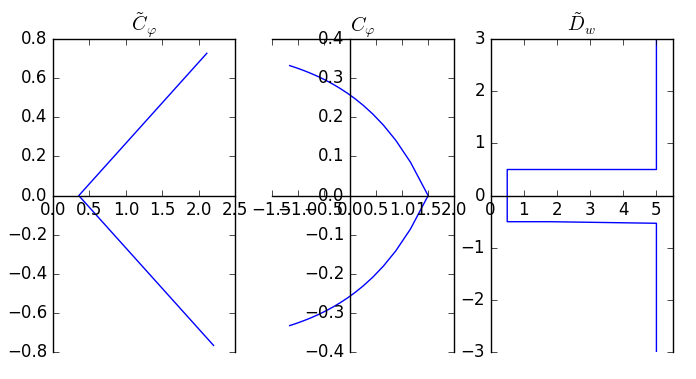
\includegraphics[width=\textwidth]{contour-cphi}
	\caption[The contours $\tilde{C}_{\varphi}$(left), $C_{\varphi}$(right) and $\tilde{D}_{w}$]
	{An illustration of the contours $\tilde{C}_{\varphi}$(left), $C_{\varphi}$(middle) for the parameter $q = 0.5$ and $\theta = 1.5$ and $\tilde{D}_{R,d}$(right) for the parameter $R = 5, d = 0.5$}
	\label{fig:cphi-contour}
\end{figure}

\begin{definition}
\label{contours-definition}
\begin{enumerate}
\item[(1)] Fix $q \in (0,1)$ and $\theta > 0$. For arbitrary but fix $\varphi \in (0, \pi / 4]$, we define the contour $\tilde{C}_{\varphi}$ to be $$\tilde{C}_{\varphi} = \{q^{\theta} + e^{i\varphi sgn(y)} |y|: y \in \mathbb{R}\}.$$ 
\item[(2)] Let $C_{\varphi}$ be the image of $\tilde{C}_{\varphi}$ under the mapping of $x \rightarrow \log_q(x)$. That is, $$C_{\varphi} = \{\log_q (q^{\theta} + e^{i\varphi sgn(y)} |y|) : y \in \mathbb{R}\}.$$
\item[(3)] For every $w \in \tilde{C}_{\varphi}$, define the contour $\tilde{D}_{w}$ to be $D_{R,d}$ as given in \textit{Section \ref{transformation-to-fd}} that it goes by straight lines from $R - i\infty$ to $R - id$, to $1/2 - id$, to $1/2 + id$, to $R + id$, and lastly to $R+i\infty$, with $R, d>0$ chosen such that the following holds:
\begin{enumerate}
\item[(a)] $arg(w(q^s-1)) \in (\pi / 2+b, 3\pi / 2 - b)$ for $b = \pi / 4 - \varphi / 2$;
\item[(b)] $q^sw$ stays to the left of $\tilde{C}_{\varphi}$ for every $s \in \tilde{D}_{w}$.
\end{enumerate}
\item[(4)] Lastly, for every $W \in C_{\varphi}$, we define the contour $D_W$ to be such that it is the contour $\tilde{D}_{q^W}$ shifted by $W$. If we let $R,d > 0$ be chosen for the contour $\tilde{D}_{q^W}$ such that the two conditions above are satisfied, then $D_W$ is defined by the straight lines going from $R+Re(W)-i \infty$ to $R+Re(W) + i(Im(W) - d)$, to $1/2+Re(W) + i(Im(W) - d)$, to $1/2 + Re(W) + i(Im(W) + d)$, to $R+Re(W) + i(Im(W) + d)$ and to $R+Re(W) + i \infty$.
\end{enumerate}

Please see \textit{Figure \ref{fig:cphi-contour}} for an illustration of the contours defined.
\end{definition}

\begin{proposition}
Fix $q \in (0,1)$, $\theta > 0$ and $\varphi \in (0, \pi / 4]$. Let $C_{\varphi}$ be defined as given in \textit{Definition \ref{contours-definition} (1)}. For every $W \in C_{\varphi}$ and the choice of $R, d$ such that the two conditions in \textit{Definition \ref{contours-definition} (3)} are satisfied with $w = q^W$. Then $$Re(W) + R > \theta.$$
\end{proposition}
\begin{remark}
An immediate result from the proposition is that there exists a $\sigma > 0$ such that $\theta + \sigma = R + Re(W)$. Moreover, the parameter $d > 0$ can be chosen to be so small such that $D_W$ and $C_{\varphi}$ do no intersect.
\end{remark}
\begin{proof}
This follows from \textit{Condition (b)} in \textit{Definition \ref{contours-definition} (3)}.
\end{proof}

We claim that with the choice of $C_{\mathbb{A}}$ to be $\tilde{C}_{\varphi}$ for any $\varphi \in (0, \pi / 4]$, and the choice of $C_{1, 2, \dots}$ to be $\tilde{D}_{w}$ for $w \in \tilde{C}_{\varphi}$, we have the convergence for the right-hand side of \textit{(\ref{continuation-equation})} as desired. To justify this, we only need to justify the three conditions in \textit{Theorem \ref{mbmb-application-to-qtasep}}, labeled as (1), (2), (3) respectively. For further details of the justification, please refer to \textit{\cite{asymptotics2013} Theorem (4.2)}.

Recall the change of variables \eqref{change-of-variables}, we have that the contour $\hat{C}_{\mathbb{A}}$ in \eqref{new-equality-mb-type} can then be chosen as $C_{\varphi}$ and that the contour $D_{R,d}^W$ for the integral kernel $\hat{K}_{\zeta}^{q-TASEP}(W,W')$ can be chosen as $D_W$. By further re-writing the kernel in the following form, we have the following result that for $x \in \mathbb{R}$, 
\begin{equation}
\label{new-equality-mb-type-2}
\mathbb{E} \left[ \frac{1}{( -q^{ \frac{\chi^{1/3}}{\log q} N^{1/3} (\xi_N - x) }; q )_{\infty}} \right] = det(I+K_x)_{L^2(C_{\varphi})},
\end{equation}
where 
\begin{align*}
& \quad K_x(W,W') \\
& = \frac{q^W \log q}{2 \pi i} \int_{D_W} \frac{dZ}{q^Z - q^{W'}} \frac{\pi}{sin(\pi (W-Z))} \frac{\exp(Nf_0(Z) + N^{2/3} f_1(Z) + N^{1/3} f_2(Z))}{\exp(Nf_0(W) + N^{2/3} f_1(W) + N^{1/3} f_2(W))},
\end{align*}
where
\begin{equation*}
f_0(Z) = -f (\log q) Z + \kappa q^Z + \log(q^Z; q)_{\infty}
\end{equation*}
\begin{equation*}
f_1(Z) = -c (\log q) Z + cq^{Z - \theta}
\end{equation*}
\begin{equation*}
f_2(Z) = \beta_x Z.
\end{equation*}

\begin{figure}
	\centering
	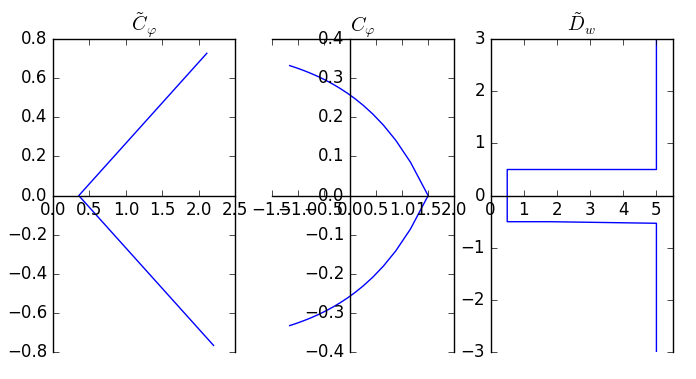
\includegraphics[width=\textwidth]{contour-cphi}
	\caption[Contour replacement of $D_W$]
	{An illustration of transformation of the contour $D_W$ mentioned in \textit{Remark \ref{circle-deformation}}}
	\label{fig:contour-dw-circle}
\end{figure}

\begin{remark}
\label{circle-deformation}
It's remarked that the contour $D_W$ in the definition of $K_x$ can be further replaced by the straight line from $R + Re(W) - i\infty$ to $R + Re(W) + i \infty$, where $R$ is the same as in the definition of $D_W$ and $d$ in the definition of $D_W$ is chose such that $D_W$ and $C_{\varphi}$ do no intersect, and some small circles surrounding the poles coming from the term $\frac{1}{sin(\pi (W - Z))}$, which are $W+1, W+2, \dots, W+k_W$ and $k_W$ denotes the total number of residues. The new contour will also be referred to as $D_W$. Please see \textit{Figure \ref{fig:contour-dw-circle}} for an illustration. 
\end{remark}

\section{Asymptotics of the Fredholm determinant}

In this section, we focus on the asymptotic behaviour of the Fredholm determinant in \eqref{new-equality-mb-type-2}. The main result is given in the following theorem.
\begin{theorem}
\label{asymptotic-theorem}
Let $x \in \mathbb{R}$ be fixed and choose $\zeta$ as in \textit{(\ref{zeta-choice})}. Then $$det(I+K_x)_{L^2(C_{\varphi})} \rightarrow F_{GUE}(x) \text{ as } N \rightarrow \infty,$$ where $F_{GUE}$ is the GUE Tracy-Widom distribution function. 
\end{theorem}

The intuition for the proof is that for $N$ large we show that the Fredholm determinants $det(I+K_x)_{L^2(C_{\varphi})}$ and $det(I-K_{Ai})_{L^2(x,\infty)}$ are arbitrarily close. To show how this can be achieved, we quote the following series of propositions from \cite{asymptotics2013} without proof and briefly explain the ideas behind. For more precise treatment, pleass refer to the original paper \cite{asymptotics2013} or \cite{phase2015}.

\begin{proposition} [\textit{\cite{asymptotics2013} Proposition (6.3)}]
\label{restriction-contour}
For any fixed $\delta > 0$ and $\epsilon > 0$ small enough, there is an $N_0$ such that $$\left| det(I+K_x)_{L^2(C_{\varphi})} - det(I+K_{x,\delta})_{L^2(C_{\varphi}^{\delta})} \right| < \epsilon$$ for all $N > N_0$ where
\begin{align*}
& \quad K_{x,\delta}(W,W') \\
& = \frac{q^W \log q}{2 \pi i} \int_{D_W^{\delta}} \frac{dZ}{q^Z - q^{W'}} \frac{\pi}{sin(\pi (W-Z))} \frac{\exp(Nf_0(Z) + N^{2/3} f_1(Z) + N^{1/3} f_2(Z))}{\exp(Nf_0(W) + N^{2/3} f_1(W) + N^{1/3} f_2(W))}
\end{align*}
and $C_{\varphi}^{\delta} = C_{\varphi} \cap \{w: |w - \theta| \le \epsilon \}$, $D_W^{\delta} = D_W \cap \{z: |z - \theta| \le \delta\}$.
\end{proposition}

This proposition essentially says that the asymptotically contribution to the Fredholm determinant outside any neighbourhood of $\theta$ can be ignored. Therefore, we only need to deal with the behavior of the Fredholm determinant around a small neighborhood of $\theta$. With this, the contour $C_{\varphi}$ and $D_{W}$ can be localized to a small neighborhood of $\theta$ (that is, $C_{\varphi}^{\delta}$ and $D_{W}^{\delta}$ respectively) without affecting the asymptotic behaviour of the determinant.

We then perform the following deformation of the contour $C_{\varphi}^{\delta}$ and $D_W^{\delta}$. Using Cauchy theorem, we are able to deform the contour $C_{\varphi}^{\delta}$ to $\{\theta + |y|e^{i(\pi - \tilde{\varphi}) sgn(y)}: y \in [-\delta, \delta]\}$ with some $\tilde{\varphi} \in (0, \pi / 2)$ chosen such that the two contours have the same endpoint. Similarly, we deform the straignt line $R+Re(W) + i \mathbb{R}$ in the contour $D_W^{\delta}$ to be $D_{\varphi}^{\delta} = \{\theta + |t| e^{i \varphi sgn(t)}: t \in [-\delta, \delta] \}$ if the $R$ in the definition of $D_W$ is chosen such that the two endpoints of the two contours coincide. 

After the above deformation, we introduce the following change of variables to $W, W'$ and $Z$: $$W = \theta + wN^{-1/3}, W' = \theta + w' N^{-1/3}, Z = \theta + zN^{-1/3}.$$ From the relationship, we get the corresponding contours for $w, w'$ and $z$ to be $C_{\varphi,\delta N^{1/3}}$ and $D_{\phi, \delta N^{1/3}}$, where
$$C_{\varphi,L} = \{|y|e^{i(\pi - \tilde{\varphi}) sgn(y)}: y \in [-L, L]\}, D_{\varphi, L} = \{|t| e^{i \varphi sgn(t)}: t \in [-L, L]\}$$ for $L \in (0, \infty].$ To be explicit, we have the following: $$det(I+K_{x, \delta})_{L^2(C_{\varphi}^{\delta})} = det(I +K_{x, \delta}^N )_{L^2(C_{\varphi, \delta N^{1/3}})},$$ where 
\begin{equation}
\label{rescaled-kernel}
K_{x, \delta}^N(w,w') = N^{-1/3} K_{x, \delta N^{1/3}} (\theta + wN^{-1/3}, \theta + w'N^{-1/3}).
\end{equation}

Moreover, from the definition of $f_0(Z), f_1(Z), f_2(Z)$, we have the following Taylor expansion of each of them around a neighborhood of $\theta$:
\begin{itemize}
\item $f_0(Z) = f_0(\theta) + \frac{\chi}{3} (Z - \theta)^3 + \mathcal{O}((Z - \theta)^4)$
\item $f_1(Z) = f_1(\theta) + \frac{c(\log q)^2}{2} (Z - \theta)^2 + \mathcal{O}((Z - \theta)^3)$
\item $f_2(Z) = f_2(\theta) + \beta_x (Z - \theta)$
\end{itemize}
Substituting these into (\ref{rescaled-kernel}), we can transform the kernel into the following explicit form as stated in the following proposition.

\begin{proposition} [\textit{\cite{asymptotics2013} Proposition (6.4)}]
Let $\varphi \in (0, \pi / 2)$ be sufficiently closed to $\pi / 2$ and let $\epsilon > 0$ be fixed. There is a small $\delta > 0$ and an $N_0$ such that for any $N > N_0$, $$|det(I +K_{x, \delta}^N )_{L^2(C_{\varphi, \delta N^{1/3}})} - det(I + K'_{x, \delta N^{1/3}})_{L^2(C_{\varphi, \delta N^{1/3}})}| < \epsilon,$$ where $$K'_{x,\delta N^{1/3}}(w,w') = \frac{1}{2 \pi i} \int_{D_{\varphi, \delta N^{1/3}}} \frac{dz}{(z-w')(w-z)} \frac{e^{\chi z^3 / 3 + c (\log q)^2 z^2 / 2 + \beta_x z}}{e^{\chi w^3 / 3 + c (\log q)^2 w^2 / 2 + \beta_x w}}.$$
\end{proposition}

The reason why we can choose $\varphi$ that is originally in $(0, \pi / 4]$ to be close to $\pi / 2$ is because of the following proposition.
\begin{proposition} [\textit{\cite{asymptotics2013} Proposition (6.2)}]
For fixed $q \in (0,1), \theta > 0$ and $N$ large enough, the contour $C_{\varphi}$ with $\varphi \in (0, \pi / 4)$ for the kernel $K_x$ can be extended to any $\varphi \in (0, \pi / 2)$ without affecting the Fredholm determinant $det(I+K_x)_{L^2(C_{\varphi})}$.
\end{proposition}

The following proposition asserts that we can expand the bound on the contour $D_{\varphi, \delta N^{1/3}}$ to $D_{\varphi, \infty}$. Similar to \textit{Proposition \ref{restriction-contour} }, we are essentially saying that asymptotically the only part of the contour that contributes to the Fredholm determinant is the part around some neighborhood of $0$. It is made precise by the following:

\begin{proposition} [\textit{\cite{asymptotics2013} Proposition (6.5)}]
As $N \rightarrow \infty$, we have $$det(I+K'_{x, \delta N^{1/3}})_{L^2(C_{\varphi, \delta N^{1/3}})} \rightarrow det(I+K'_{x, \infty})_{L^2(C_{\varphi, \infty})}.$$
\end{proposition}

And lastly, the kernel $K'_{x, \infty}$ can be reformulated to the Airy kernel via the following proposition.
\begin{proposition} [\textit{\cite{asymptotics2013} Proposition (6.6)}]

$$det(I+K'_{x,\infty})_{L^2(C_{\varphi, \infty})} = det(I - K_{Ai, x})_{L^2(\mathbb{R}_+)}.$$
\end{proposition}

By the definition of the GUE Tracy-Widom distribution introduced at the beginning of the chapter, we therefore conclude \textit{Theorem \ref{asymptotic-theorem}}.

\section{Distribution of the rescaled fluctuation}
In the last section, we concluded with \textit{Theorem \ref{asymptotic-theorem}} that for $N$ large, $det(I+K_x)_{L^2(C_{\varphi})} \rightarrow F_{GUE}(x)$. Therefore, 
\begin{equation}
\label{finale-equality}
\mathbb{E} \left[ \frac{1}{( -q^{ \frac{\chi^{1/3}}{\log q} N^{1/3} (\xi_N - x) }; q )_{\infty}} \right] \rightarrow F_{GUE}(x) \text{ as } N \rightarrow \infty.
\end{equation}
Define $f_N(y) = (-q^{\frac{\chi^{1/3}}{\log q} N^{1/3} y};q)_{\infty}^{-1}.$ Then we have that $$\mathbb{E} \left[ \frac{1}{( -q^{ \frac{\chi^{1/3}}{\log q} N^{1/3} (\xi_N - x) }; q )_{\infty}} \right] = \mathbb{E} \left[ f_N(\xi_N - x) \right].$$ We observe the following facts about $f_N(y)$:
\begin{itemize}
\item $f_N(y)$ is a mapping from $\mathbb{R}$ to $[0,1]$.
\item For each $N$, $f_N(y)$ is strictly decreasing on $y$. This is because $\log q < 0$ for $q \in (0,1)$. Moreover, $\lim_{y \rightarrow \infty} f_N(y) = 1$ and $\lim_{y \rightarrow -\infty} f_N(y) = 0$.
\item For each $\delta > 0$, on $\mathbb{R} \setminus [-\delta, \delta]$, the sequence of functions $f_N$ converges uniformly to $\mathbbm{1}(y < 0)$.
\end{itemize}
The last observation follows from the fact that $\frac{1}{1+q^{\frac{\chi^{1/3}}{\log q} N^{1/3} y + k}}$ is uniformly close to $1$ if $y \in (\delta, \infty)$ and $0$ if $y \in (-\infty, -\delta)$.

To continue our discussion, we quote the following lemma from \textit{\cite{macdonald2014} Lemma 4.1.39 }. 
\begin{lemma}
\label{last-lemma}
Consider a sequence of functions $(f_n)_{n \ge 1}$ mapping $\mathbb{R} \rightarrow [0,1]$ such that for eaach $n$, $f_n(y)$ is strictly decreasing in $y$ with a limit of $1$ at $y = -\infty$ and $0$ at $y = \infty$, and for each $\delta > 0$, on $\mathbb{R} \setminus [-\delta, \delta]$, $f_n$ converges uniformly to $\mathbbm{1}(y < 0)$. Consider a sequence of random variables $X_n(t)$ such that for each $r \in \mathbb{R}$, $$\mathbb{E} [f_n(X_n - r)] \rightarrow p(r)$$ and assume that $p(r)$ is a continuous probability distribution function. Then $X_n$ converges weakly in distribution to a random variable $X$ which is distributed according to $\mathbb{P}(X < r) = p(r)$.
\end{lemma}

Combining the lemma above, the observations about $f_N(y)$ and (\ref{finale-equality}), we conclude the following theorem.
\begin{theorem}
Let $q \in (0,1)$ and $\theta > 0$ be fixed. For any $c, x \in \mathbb{R}$, we have that $$\lim_{N \rightarrow \infty} \mathbb{P}(\xi_N < x) = F_{GUE}(x),$$ where $$\xi_N = \frac{X_N(\tau(N,c)) - p(N,c)}{\chi^{1/3} (\log q)^{-1} N^{1/3}}.$$
\end{theorem}
\begin{proof}
The proof is by applying Lemma \ref{last-lemma} directly with the sequence of functions $f_N(y)$.
\end{proof}
\appendix
\chapter{Tables}

\begin{table}
\caption{Armadillos}
\label{arm:table}
\begin{center}
\begin{tabular}{||l|l||}\hline
Armadillos & are \\\hline
our	   & friends \\\hline
\end{tabular}
\end{center}
\end{table}

\clearpage
\newpage

\chapter{Figures}

\vspace*{-3in}

\begin{figure}
\vspace{2.4in}
\caption{Armadillo slaying lawyer.}
\label{arm:fig1}
\end{figure}
\clearpage
\newpage

\begin{figure}
\vspace{2.4in}
\caption{Armadillo eradicating national debt.}
\label{arm:fig2}
\end{figure}
\clearpage
\newpage

%% This defines the bibliography file (main.bib) and the bibliography style.
%% If you want to create a bibliography file by hand, change the contents of
%% this file to a `thebibliography' environment.  For more information 
%% see section 4.3 of the LaTeX manual.
\begin{singlespace}
\bibliography{main}
\bibliographystyle{plain}

\begin{thebibliography}{9}

\bibitem{duality2014}
  A.Borodin, I. Corwin, and T. Sasamoto,
  \emph{From duality to determinants for q-TASEP and ASEP},
  Annals of Probability 2014,
  Vol. 42, No. 6, 2314-2382,
  2014,
  arXiv:1207.5035.

\bibitem{macdonald2014}
  A.Borodin, I. Corwin,
  \emph{Macdonald processes},
  Probability Theory and Related Fields,
  2014,
  arXiv:1111.4408.

\bibitem{generator-duality}
  A. Vo\ss -B\"o hme, W. Schenk and A.-K. Koellner,
  \emph{On the equivalence between Liggett duality of Markov processes and the duality relation between their generators},
  Markov Processes and Related Fields,
  2011

\bibitem{phase2015}
  G. Barraquand,
  \emph{A phase transition for q-TASEP with a few slower particles},
  Stochastic Processes and Their Applications 125 (2015),
  pp. 2674-2699,
  2015,
  arXiv:1404.7409.

\bibitem{symmetrization}
  I.G. Macdonald,
  \emph{Symmetric functions and Hall polynomials},
  2nd edition, 
  Oxford University Press,
  New York,
  1999

\bibitem{interacting-particle-system}
  Liggett, T. M.,
  \emph{Interacting Particle Systems},
  Springer,
  Berlin,
  2005,
  MR2108619.

\bibitem{asymptotics2013}
  P. L. Ferrari, B. Vet\H o,
  \emph{Tracy-Widom asymptotics for q-TASEP},
  Ann. Inst. H. Poincar\' e Probab. Stat.,
  2013,
  arXiv:1310.2515.

\end{thebibliography}

\end{singlespace}

\end{document}

